
\documentclass[preprint,10pt,times]{elsarticle}
\usepackage{geometry}
 \geometry{
 b4paper,
 total={160mm,257mm},
 right=80mm,
 top=20mm,
 }


\usepackage{ulem}
\usepackage{color,soul}

\setul{0.5ex}{0.3ex}
\definecolor{Green}{rgb}{0,1,0}
\setulcolor{Green}


\definecolor{Red}{rgb}{1,0.0,0.0}
\setulcolor{Red}


\definecolor{Blue}{rgb}{0,0.0,1}
\setulcolor{Blue}


\usepackage[cal=boondox,scr=boondoxo]{mathalfa}
\DeclareFontEncoding{FML}{}{}
\DeclareFontSubstitution{FML}{fncmi}{m}{it}
\DeclareSymbolFont{fourierletters}{FML}{fncmi}{m}{it}
\SetSymbolFont{fourierletters}{normal}{FML}{fncmi}{m}{it}
\DeclareMathSymbol{\fP}{\mathalpha}{fourierletters}{`E}
\DeclareSymbolFont{Nperm}{OML}{cmss}{bx}{it}

\SetSymbolFont{Nperm}{bold}{OML}{cmss}{bx}{it}
\DeclareMathSymbol{\nw}{\mathalpha}{Nperm}{`w}
\newcommand{\unit}[1]{\ensuremath{\, \mathrm{#1}}}


\usepackage{amssymb,amsmath,gensymb,amsthm,mathtools}
\newtheorem{theorem}{Theorem}[section]
\usepackage{lineno}
%\linenumbers

\usepackage{tabularx}
\numberwithin{equation}{section}
% \usepackage{showkeys}
% \usepackage{xcolor}

\pagecolor[rgb]{0.6,0.6,0.6} %black



\usepackage[T1]{fontenc}
% \usepackage{cite}
\usepackage{tikz}
\newcommand*\circled[1]{\tikz[baseline=(char.base)]{
\node[shape=circle,draw,inner sep=1pt] (char) {#1};}}


\usepackage{enumitem}
\usepackage{pifont}% http://ctan.org/pkg/pifont
\newcommand{\cmark}{\ding{51}}%
\newcommand{\xmark}{\ding{55}}%
\usepackage{epstopdf}
\usepackage{xr}
\usepackage{hyperref}
\hypersetup{
colorlinks = true,
citecolor = blue,
linkcolor = blue
}

\newcommand{\tbp}[1]{\tilde{{\mathpzc{#1}}}}
\newcommand{\bp}[1]{{\mathpzc{#1}}}


%\usepackage{breqn}
\newcommand{\pd}[2]{\frac{\partial #1}{\partial #2}}
\newcommand{\stophere}[2]{{\color{#1} $\blacksquare$  \color{#1}#2} }
\newcommand{\comment}[1]{}


%\renewcommand{\comment}[2]{{\color{#1} $\blacksquare$ \footnote{\noindent \color{#1}#2} }}
\newcommand{\commenti}[2]{{\color{#1} $\blacksquare$  \color{#1}#2} }
\newcommand{\commentm}[2]{{\color{#1} $\blacksquare$  \marginpar{\color{#1}#2} }}



% Special font for physical quantities
\newcommand{\forcemag}{f}
\newcommand{\physF}{\boldsymbol{\mathfrak{f}}} %
\newcommand{\physB}{\mathscr{b}} % Width of the thin film
\newcommand{\physE}{{\mathpzc{E}}}
\newcommand{\ndE}{E}
\newcommand{\ndL}{L}
\newcommand{\physI}{{\mathscr{I}}}
\newcommand{\ndI}{I}
\newcommand{\physkc}{\mathscr{k}_{\rm c}}
\newcommand{\ndkc}{k_{\rm c}}
\newcommand{\physh}{\mathscr{h}} %
\newcommand{\physe}{\hat{\mathbscr{e}}} %
\newcommand{\physf}{\hat{\boldsymbol{\mathfrak{f}}}}
\newcommand{\physm}{\mathscr{m}} %
\newcommand{\physu}{\mathbscr{u}}
\newcommand{\physw}{\mathscr{w}}
\newcommand{\rtple}[1]{\boldsymbol{#1}}
\newcommand{\n}{\mathfrak{n}} %

\newcommand{\physwc}{\bm{w}_c}
\newcommand{\physws}{\bm{w}_s}
\newcommand{\physwo}{\bm{w}_0}

\renewcommand{\u}[1]{\boldsymbol{#1}}
\newcommand{\OriginRefEucldPtSpace}{O_{\mathrm{ R}}}
\newcommand{\MapManifoldToRefEucldPtSpace}{\kappa_{\mathrm{ R}}}
\renewcommand{\t}[1]{\tilde{#1}}
\renewcommand{\b}[1]{\mathbb{#1}}
\renewcommand{\c}[1]{\mathcal{#1}}
\newcommand{\lsc}[2][\mathscr{l}]{{}^{ #1 }\! #2}
\newcommand{\lscH}[1]{\lsc[H]{#1}}
\newcommand{\dsf}[1]{\Delta\boldsymbol{\mathsf #1}}
\newcommand{\tpsb}[1]{\left. #1 \right.^{\mathsf T}}
\newcommand{\tps}[1]{\left( #1 \right)^{\mathsf T}}
\newcommand{\usf}[1]{\u{\mathsf #1}}
\newcommand{\busf}[1]{\bar{\usf{ #1}}}
\newcommand{\tu}[1]{\tilde{\u{ #1}}}
\newcommand{\tusf}[1]{\tilde{\usf{ #1}}}
\newcommand{\btusf}[1]{\bar{\tusf{ #1}}}
\newcommand{\pr}[1]{\left( #1 \right)}
\newcommand{\spr}[1]{\left[ #1 \right]}
\newcommand{\encl}[1]{\left. #1 \right.}
\newcommand*{\subfigurewdith}{0.8\textwidth}
\newcommand{\D}[1]{D\hspace{-.1em}#1}
\newcommand{\Dr}{D\hspace{-.1em}\varrho}
\newcommand{\Drp}{\Dr^{+}}
\newcommand{\Drm}{\Dr^{-}}
\newcommand{\Dro}{\dot{\rho}}
\newcommand{\DDro}{\ddot{\rho}}
\newcommand{\Df}{\dot{f}}
\newcommand{\DDf}{\ddot{f}}
\newcommand{\Drop}{\Dro^{+}}
\newcommand{\Drom}{\Dro^{-}}
\newcommand{\Dl}{\dot{l}}
\newcommand{\Da}{\dot{a}}
\newcommand{\DDl}{\ddot{l}}
\newcommand{\DF}{\dot{F}}
\newcommand{\DDF}{\ddot{F}}
\newcommand{\Dlp}{\Dl^{+}}
\newcommand{\Dlm}{\Dl^{-}}
\newcommand{\Dam}{\Da^{-}}
\newcommand{\Deq}{\mathcal{D}^{\circ}}
\newcommand{\Dst}{\mathcal{D}^{\stable}}
\newcommand{\Dnt}{\mathcal{D}^{\odot}}
\newcommand{\Dunst}{\mathcal{D}^{\otimes}}
\newcommand{\conf}{\boldsymbol{\kappa}}
\newcommand{\confp}{\tilde{\boldsymbol{\kappa}}}
\newcommand{\p}{\,\mathsf{p}}
\newcommand{\Inv}{\,\mathsf{Inv}}





\newcommand{\hlc}[2][yellow]{ {\sethlcolor{#1} \hl{#2}} }
\usepackage{wrapfig}




% \usepackage{amsmath}
% \usepackage[small]{eulervm}
  \DeclareMathAlphabet{\mathvz}{OT1}{LinuxBiolinumT-OsF}{m}{sl}

  \DeclareMathAlphabet{\mathlib}{OT1}{LinuxLibertineT-OsF}{m}{it}
  \DeclareMathAlphabet{\mathbio}{OT1}{LinuxBiolinumT-OsF}{m}{it}
\DeclareMathAlphabet{\mathpzc}{OT1}{pzc}{m}{it}





\usepackage[prefix=sol]{xcolor-solarized}
\usepackage{booktabs}
\usepackage{float}
% \usepackage{mathptmx}
\usepackage{pdflscape}
\usepackage{threeparttable}
\usepackage{tabto}

\usepackage{sectsty}
 \sectionfont{\fontsize{16}{16}\selectfont}

%CUSTOM COMMANDS
\newcommand{\norm}[1]{\ensuremath \lVert #1 \rVert}
\newcommand{\bs}[1]{\ensuremath{\mathbf{#1}}}
\newcommand{\pD}[2]{\frac{\partial #1}{\partial #2}}
\renewcommand{\D}[2]{\frac{\mathrm{d} #1}{\mathrm{d} #2}}
\newcommand{\dx}[1]{\,\mathrm{d} #1}
\newcommand{\ex}{{\bm{\hat{e}}}_1}
\newcommand{\ey}{{\bm{\hat{e}}}_2}
\newcommand{\ez}{{\bm{\hat{e}}}_3}
\newcommand{\ei}{{\bm{\hat{e}}}_i}
\newcommand{\ej}{{\bm{\hat{e}}}_j}
\newcommand{\er}{{\bm{\hat{e}}}_r}
\newcommand{\et}{{\bm{\hat{e}}}_\theta}
\newcommand{\ep}{{\bm{\hat{e}}}_\phi}
\usepackage{xspace}
\newcommand{\TA}{\textit{Ta.\@}\xspace}
\newcommand{\EA}{\textit{Ea.\@}\xspace}
\newcommand{\subf}[1]{\pr{\textsf{#1}}}
\newcommand{\ra}[1]{\renewcommand{\arraystretch}{#1}}
\newcommand{\idp}{\mathsf{p}}







\newcommand{\notimplies}{%
  \mathrel{{\ooalign{\hidewidth$\not\phantom{=}$\hidewidth\cr$\implies$}}}}



\usepackage[obeyFinal]{todonotes}
\setlength\marginparwidth{2.5in}
\renewcommand{\>}{$\Rightarrow$}


%\usepackage[nomarkers,figuresonly]{endfloat}

\usepackage{algorithm,algorithmicx}
\usepackage{algpseudocode}
\usepackage[hang,flushmargin]{footmisc}
\DeclareMathOperator*{\argmin}{arg\,min} % Jan Hlavacek


\usepackage{xspace}
\newcommand\bmmax{0}
\usepackage{bm}

\journal{International Journal of Solids and Structures}
\begin{document}
\begin{frontmatter}

%% Title, authors and addresses

%% use the tnoteref command within \title for footnotes;
%% use the tnotetext command for theassociated footnote;
%% use the fnref command within \author or \address for footnotes;
%% use the fntext command for theassociated footnote;
%% use the corref command within \author for corresponding author footnotes;
%% use the cortext command for theassociated footnote;
%% use the ead command for the email address,
%% and the form \ead[url] for the home page:
%% \title{Title\tnoteref{label1}}
%% \tnotetext[label1]{}
%% \author{Name\corref{cor1}\fnref{label2}}
%% \ead{email address}
%% \ead[url]{home page}
%% \fntext[label2]{}
%% \cortext[cor1]{}
%% \address{Address\fnref{label3}}
%% \fntext[label3]{}

\title{Effective bending stiffness of multilayered composite cylinders with cylindrical orthotropy}

%% use optional labels to link authors explicitly to addresses:
%% \author[label1,label2]{}
%% \address[label1]{}
%% \address[label2]{}

\author{Wenqiang Fang, Weilin Deng, Haneesh Kesari}

\address{School of Engineering,	Brown University, Providence, RI 02912}

\begin{abstract}
%% Text of abstract
A wide range of structural biomaterials are multilayered composite cylinders where each layer is made of cylindrical orthotropic materials. The paper presents analytical expressions for the asymptotic bending stiffness of such structures by performing asymptotic analysis of the bending stiffness formula obtained by Jolicoeur and Cardou [Jolicoeur, C., Cardou, A. (1994): \textit{J. Eng. Mech.} 120, 2556–2574]. In our analysis, different interfacial conditions between layers, such as perfectly bonded and frictionless interfaces, are considered.
We also explore the effects of heterogeneity on the structure's bending stiffness by
altering the stacking orientations of the laminae of the structure.
Our studies reveal that the bending stiffness of perfectly bonded multilayered cylindrical structures consisting of heterogeneous materials could be higher than that of structures made up with the corresponding constituent material.
The results shed light on the role of multilayered structures with cylindrical orthotropy in structural biomaterials.

\end{abstract}

\begin{keyword}
%% keywords here, in the form: keyword \sep keyword
Multilayered composite structure \sep Cylindrical orthotropy \sep Effective bending stiffness \sep asymptotic analysis

%% PACS codes here, in the form: \PACS code \sep code

%% MSC codes here, in the form: \MSC code \sep code
%% or \MSC[2008] code \sep code (2000 is the default)

\end{keyword}

\end{frontmatter}

\linenumbers

%% main text
\section{Introduction}
\label{sec:intro}
TESTING

%Many structural biomaterials achieve outstanding macroscale mechanical properties such as strength, stiffness, and toughness through the geometric arrangement of their constituent components at the microscale~\cite{meyers2013structural}. Such examples of microstructural complexity is the multilayered structures with helical symmetry found in the osteon of bone~\cite{wegst2015bioinspired}, artery walls~\cite{Gasser2006}, the wall structures of wood~\cite{Fratzl2007} and bamboo~\cite{wai1985morphological}, and sea sponge skeletons~\cite{Aizenberg2005} etc (Fig.~\ref{fig:Laminatedbiomaterials}). The multilayered structures with helical symmetry are also found in materials such as multi-walled nanotube~\cite{Delgado2008} and filament-wound composite pipes. The macroscale performances of multilayered structures are determined by the microscale properties of individual layers, the interface between the layers, and the layer arrangement. Therefore the understanding of connections between the macroscale properties and micro structures is useful to guide the design of biologically inspired materials with tailorable properties.

Structural biomaterials such as mother of pearl (nacre)~\cite{jackson1988mechanical}, spicules~\cite{monn2015new}, and bones~\cite{wegst2015bioinspired} are of growing interest in material and mechanics communities.
%
They are composites that mainly consists of a stiff mineral phase which is often in the form of platelets~\cite{currey1977mechanical, meyers2008biological, espinosa2011tablet} or fibers~\cite{Aizenberg2005, zhang2011structure, li2015hierarchical}, and contributes to~$95\%$ of the materials volumes.
%
The platelets and fibers are glued to the mineral phase through a compliant organic phase.
%
These natural composites are distinguished from their synthetic counterparts by the facts that their effective properties at the macro scale, such as strength and fracture toughness, are quite high despite the corresponding properties of their constituent phases being very poor.
% \ul{phases being very poor.}\todo[fancyline]{English. "being very poor"}
%
\setulcolor{green}\textcolor{red}{For example, the tensile strength of the spicules of the sponge \textit{Euplectella aspergillum} is much higher than the silicate glass fiber~\cite{walter2007mechanisms}.}\marginpar{}
%
Nacre can achieve relatively high fracture toughness 20-30 times that of pure aragonite~\cite{tang2007elasto, barthelat2007experimental}.
%
With such remarkable mechanical performances, structural biomaterials can serve as fascinating model material systems for the discovery of new mechanics of materials principles.
%


The remarkable enhancement in the structural biomaterials' macro-scale properties in comparison to their micro-scale properties is believed to be due to the highly organized and quite elaborate architecture in which the mineral phases is interlaid with the organics phase.
A number of studies have been performed to delineate the mechanical principles that quantitatively capture the relationship between large-scale mechanical properties and small-scale architecture.
%
In most of those studies the focus has been on the brick-mortar architecture which can be described as a ordered stacking of thin flat platelets.
%
For example, Gao and co-workers~\cite{gao2006application, ji2010mechanical} developed a multi-level staggered mechanical (tension-shear chain) model for a self-similar bone to understand the role of hierarchical structures of bone.
%
Bertoldi et al.~\cite{bertoldi2008nacre} derived the effective stiffness tensor of nacre based on the tension-shear chain model through the homogenization technique and showed that nacre was orthotropic and had different Young's modulus when in tension and compression.
%
Rim et al.~\cite{rim2011dimensional} performed a parametric analysis to investigate the effect of the microstructure geometry on the nacre-inspired composite's strength and toughness.
%
Begley et al.~\cite{begley2012micromechanical} developed a micromechanical model to evaluate the effective properties of the brick-mortar composite, such as elastic modulus, strength and work-to-failure.
%
Shao et al.~\cite{shao2012discontinuous} presented a microstructure-based fracture mechanics model to study the toughening effect due to the crack-bridging mechanism of platelets in nacre.
%



However, there exist a large number of structural biomaterials with cylindrical structures and displaying a helical symmetry.
%
Representative examples include the Ponderosa pine~\cite{leelavanichkul2004grain}, the sea sponge skeletons~\cite{Aizenberg2005}, and the tusk of the narwhal~\cite{kingsley1988spiral}, as shown in Fig.~\ref{fig:Laminatedbiomaterials}~$\subf{A-C}$.
%
Furthermore, some other helical structural biomaterials are often found to have the architecture consisting of a co-axial array of thin annular layers, which is referred to multilayered composite structure.
%
This multilayered helical structure is observed in the osteon of bone~\cite{wegst2015bioinspired}, the artery wall~\cite{Gasser2006}, and the wood's cell wall~\cite{Fratzl2007} etc. (see Fig.~\ref{fig:Laminatedbiomaterials}~$\subf{D-F}$).
%
Some engineering materials such as multiwalled carbon nanotube (see Fig.~\ref{fig:Laminatedbiomaterials}~$\subf{G}$) and filament-wound composite pipes have multilayered helical structure as well.
%
Although the property-structure connection of biomaterials with brick-mortar architecture has been extensively studied, the relationship between the effective mechanical properties and the small-scale architectures for structural biomaterials consisting of cylindrical layers with helical symmetries is much elusive.
%
\begin{figure}[t]
    \centering
    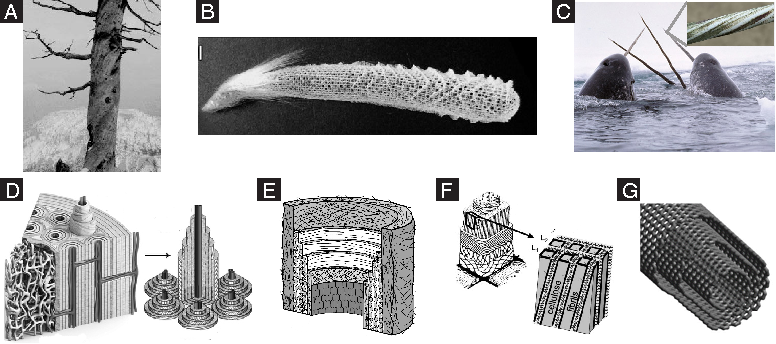
\includegraphics[width=0.9\textwidth]{../LyxFiles/figure/Laminatedbiomaterials.pdf}
    \caption{Representative examples of structures displaying a helical symmetry.
~$\subf{A}$ Ponderosa pine (modified with permission from~\cite{leelavanichkul2004grain}),
~$\subf{B}$ the sea sponge skeletons (reprinted from~\cite{monn2015new}),
~$\subf{C}$ the tusk of the narwhal (image courtesy Glenn Williams),
~$\subf{D}$ the osteon microstructure of bone (modified with permission from~\cite{Buckwalter1995Bone}),
~$\subf{E}$ the artery wall (modified with permission from~\cite{Gasser2006}),
~$\subf{F}$ the wood's cell wall (modified with permission from~\cite{Fratzl2007}),
   and~$\subf{G}$ multiwalled carbon nanotube (modified with permission from~\cite{Delgado2008}).}
    \label{fig:Laminatedbiomaterials}
\end{figure}
%


Most of the multilayered structural biological and engineering composite materials are essentially anisotropic and heterogeneous.
Moreover, the helical symmetric layers of the structures are cylindrical orthotropic.
%
Understanding and analyzing the overall deformation of such materials with multilayered anisotropic cylindrical microstructures requires the knowledge of their effective (i.e., homogenized) elastic properties, which can be obtained through the anisotropic elasticity theory and homogenization theory.
%
The theory of anisotropic elasticity in the cylindrical coordinates system is developed and summarized in monographs by~\cite{Lekhnitskii1981,Ting1996anisotropic}.
%
Analytical solutions for displacement and stress analysis of anisotropic composite cylinders subjected to typical loading conditions such as tension, shear, torsion, pressuring, thermal deformation and bending are extensively studied, for example, see~\cite{kollar1992stress,kollar1992composite, Jolicoeur1994, ting1996pressuring, chen2000revisit, tarn2001laminated, huang2001analysis,xia2002bending,crossley2003analytical,tsukrov2010elastic} etc. Inspired by those analytical solutions, a recent study by Gnoli et al.~\cite{gnoli2020homogenization} compared the stiffnesses of the fiber-reinforced cylinder composite beams with various lamination schemes. One interesting observation is that all stiffness constants seem to become stable when three or four layers are considered in the composite beams.
%One approach to investigate the macroscale effective properties is the standard asymptotic homogenization method, a two-scale technique that uses asymptotic expansions of displacement and stress fields and appropriate variational principles to analyze characteristics of heterogeneous materials, cf. the monographs by~\cite{bensoussan2011asymptotic} and~\cite{sánchez1980nonhomogeneous} and recent reviews by~\cite{kalamkarov2009asymptotic},~\cite{pindera2009micromechanics}, and~\cite{charalambakis2010homogenization}.
%
%\stophere{cyan}{Two ways to obtain homogenized bending stiffness: homogenized elastic constants, or infinite layer numbers}
%
%\stophere{cyan}{Literature survey on homogenization of composite materials.}
% %

Regarding the homogenization of multilayered cylindrical structures, Chatzigeorgiou et al.~\cite{chatzigeorgiou2008homogenization} studied the homogenized elastic coefficients of an anisotropic hollow layered tube with discontinuous elastic constants under axisymmetric loading condition. They~\cite{chatzigeorgiou2012effective} also proposed a modified asymptotic expansion homogenization method to compute effective thermomechanical properties of composites with periodicity in cylindrical coordinates.
%
By taking into account the discontinuous stress and strain distributions in each layer, Sun et al.~\cite{sun2014homogenization,sun2014stress} proposed a force-displacement equivalence method to determine the homogenized elastic constants of general multilayered composite cylindrical structures with curvilinear orthotropy. However, the lack of asymptotic analysis makes their method too complicated to apply in practice since the formulations involves the number of layers in the cylindrical composite.

In this paper we derive analytical expressions for the asymptotic bending stiffness of multilayered composite cylinderss with cylindrical orthotropy by performing asymptotic analysis on the bending stiffness formula obtained by Jolicoeur and Cardou~\cite{Jolicoeur1994}.
%
Both the interfacial conditions between adjacent layers and the lamination schemes of the layers are considered.
%
It is found that the effective bending stiffness of multilayered cylindrical orthotropic structure with frictionless interfaces converges as the number of layers become infinity. %
Furthermore, the asymptotic bending stiffness of perfectly bonded multilayered cylindrical structures consisting of heterogeneous materials is higher than that of structures made of either constituent material.


The paper is organized as follows:~$\S$\ref{sec:bending_model} describes the model problem of pure bending of multilayered cylindrical structures and summaries the results obtained by Jolicoeur and Cardou.~$\S$\ref{sec:limit_analysis} presents the asymptotic analysis procedures of bending stiffness of the structure. The expressions of asymptotic bending stiffness for different interfacial conditions and lamination schemes are derived.~$\S$\ref{sec:discussion} illustrates the numerical examples and discussions of the results. The final section includes the major conclusions.



%%%%%%%%%%%%%%%%%%%%%%%%%%%%%%%%%%%%%%%%%%%%%%%%%%%%%%%%%%%%%%%%%%%%%%
\section{Pure bending of multilayered composite cylinders with cylindrical orthotropy}
\label{sec:bending_model}


We consider a hollow composite cylinder consisting of~$N$ co-axial cylindrical layers and each layer is cylindrical orthotropic with different principal material property orientations (see Fig.~\ref{fig:Cylinder3D}). The inner and outer radius of the cylinder is~${}^{0}\!{r}$ and~${}^{N}\!{r}$, respectively.

We take~$\mathbb{E}$ to be a three dimensional, oriented, Hilbert space and introduce vectors~$(\physe_1,\physe_2,\physe_3)$ to form a basis for~$\mathbb{E}$. We also define an Euclidean point space~$\mathcal{E}$ as~$\mathbb{E}$'s principle homogeneous space.
The vectors~$\physe_1$,~$\physe_2$, and~$\physe_3$ are orthonormal, that is,~$\physe_i\cdot\physe_j=\delta_{ij}$, for~$i$,~$j\in (1,2,3)$, where the Kronecker delta symbol~$\delta_{ij}$ is defined as unity if~$i=j$ and zero otherwise.
Following the conventions in~\cite{rahaman2020accelerometer,deng2021angle}, we define the vectors in~$\mathbb{E}$ to have units of length, say meters, and refer to~$\mathbb{E}$ as the physical-space. The units are carried by the basis vectors~$(\physe_1,\physe_2,\physe_3)$ (see Fig.~\ref{fig:schematic}~$\subf{A}$).

We place the cylinder in~$\mathcal{E}$ so that the axis of the cylinder is aligned with~$\physe_3$ and cross sections are in~$(\physe_1,\physe2)$ plane (see Fig.~\ref{fig:schematic}~$\subf{A}$).

We also introduce a set of orthonormal vectors~$(\physe_{r}(\theta),\physe_{\theta}(\theta),\physe_{z}(\theta))$ as a basis for a global cylindrical coordinate system in~$\mathbb{E}$. The dependence of~$(\physe_{r}(\theta),\physe_{\theta}(\theta),\physe_{z}(\theta))$ on~$(\physe_1,\physe_2,\physe_3)$ is given by
\begin{subequations}
\begin{align}
\physe_{r}(\theta) & = \cos(\theta) \physe_1 + \sin(\theta) \physe_2 , \\
\physe_{\theta}(\theta) & = -\sin(\theta) \physe_1 + \cos(\theta) \physe_2 , \\
\physe_{z} (\theta) & =  \physe_3.
\end{align}
\end{subequations}

For an individual layer of material, we construct a local cylindrical coordinate system according to the principal material property orientation of the layer. We refer to the local cylindrical coordinate system as the material coordinate system. It is a rotation of the global cylindrical coordinate system through an angle~$\varphi$, the so-called helical angle, in clockwise direction with respect to the axis~$\physe_{r}(\theta)$ (see Fig.~\ref{fig:schematic}).
It can be shown in Fig.~\ref{fig:schematic}~$\subf{B}$ that $\tan(\varphi) = 2 \pi r/h$, where $h$ is the pitch height of the helix that forms the cylindrical layer. We denote the basis of the material coordinate system as~$\pr{\physf_{r}(\theta;\varphi),\physf_{\theta}(\theta;\varphi),\physf_{z}(\theta;\varphi)}$, 
% where
% \begin{subequations}
% \begin{align}
% \physf_{r} (\theta;\varphi) & =  \physe_r (\theta),\\
% \physf_{\theta} (\theta;\varphi)& = \cos(\varphi) \physe_{\theta} (\theta) - \sin(\varphi) \physe_z (\theta), \\
% \physf_{z}(\theta;\varphi) & = \sin(\varphi) \physe_{\theta} (\theta) + \cos(\varphi) \physe_z (\theta).
% \end{align}
% \end{subequations}
and the transformation matrix from~$(\physe_{r}(\theta),\physe_{\theta}(\theta),\physe_{z}(\theta))$ to~$\pr{\physf_{r}(\theta;\varphi),\physf_{\theta}(\theta;\varphi),\physf_{z}(\theta;\varphi)}$ as $\usf{Q}(\varphi)$, which can be expressed as

\begin{equation}
\usf{Q}(\varphi)
% & = \begin{bmatrix}
% \physf_{r}(\theta;\varphi)\cdot \physe_{r}(\theta) & \physf_{r}(\theta;\varphi)\cdot \physe_{\theta}(\theta) & \physf_{r}(\theta;\varphi)\cdot \physe_{z}(\theta) \\\physf_{\theta}(\theta;\varphi)\cdot \physe_{r}(\theta) & \physf_{\theta}(\theta;\varphi)\cdot \physe_{\theta}(\theta) & \physf_{\theta}(\theta;\varphi)\cdot \physe_{z}(\theta) \\\physf_{z}(\theta;\varphi)\cdot \physe_{r}(\theta) & \physf_{z}(\theta;\varphi)\cdot \physe_{\theta}(\theta) & \physf_{z}(\theta;\varphi)\cdot \physe_{z}(\theta)
% \end{bmatrix}\\& 
= \begin{bmatrix}
1 & 0 & 0 \\
 0 & \cos(\varphi) & -\sin(\varphi) \\
 0 & \sin(\varphi) & \cos(\varphi)
 \end{bmatrix}.
\end{equation}

In terms of $\usf{Q}(\varphi)$ , we have the transformation relation between~$(\physe_{r}(\theta),\physe_{\theta}(\theta),\physe_{z}(\theta))$ and~$\pr{\physf_{r}(\theta;\varphi),\physf_{\theta}(\theta;\varphi),\physf_{z}(\theta;\varphi)}$ as
\begin{equation}
\physf_{i} (\theta;\varphi) = \sum_{j \in \mathcal{I} } Q_{ij}(\varphi)\physe_{j}(\theta), \quad \text{for} \,i \in \mathcal{I} ,
\label{eq:Qtransform}
\end{equation}
where $\mathcal{I} :=\pr{r,\theta,z}$,  $Q_{ij}(\varphi) = \pr{\usf{Q}(\varphi)}_{ij}$ are elements of the matrix $\usf{Q}(\varphi)$.

% ,~$\physe_3$ is the longitudinal direonction making an angle~$\varphi$, the so-called helical angle, with the cylinder axis, and the direction perpendicular to~$\physe_3$ and~$\physe_1$ is defined as tangential direction~$\physe_2$.

The solution of a single cylinder with cylindrical orthotropy subjected to pure bending was obtained by Lekhnitskii~\cite{Lekhnitskii1981}. Jolicoeur and Cardou extended this method to a more general bending problem of a co-axial array of~$N$ cylindrical layers with cylindrical orthotropy. Each cylindrical layers have different helical angles (see Fig.~\ref{fig:schematic}~$\subf{B}$). The interfaces between adjacent layers could be either perfectly bonded or frictionless. The elastic problem is solved by using stress function method with assumptions that the elastic cylinder is under small strains, the loads along~$z$-axis are constant, no shear load resultant, and stresses and strains only depend on~$r$ and~$\theta$, which implies constant curvature of the bent cylinder. In the following, we describe the generalized Hooke's law of cylindrical orthotropy in~$\S$\ref{sec:MatrixTrans}. The results that are obtained by Jolicoeur and Cardou and relevant to the pure bending problem are summarized in~$\S$\ref{sec:bending stiffness}.


\begin{figure}[t]
  \centering
  \graphicspath{{../LyxFiles/figure/}}
  \includegraphics[width=0.8\textwidth]{Cylinder3D_V2.pdf}
  \caption{Three-dimensional schematics of  $N$-layer cylindrical structure.~$\subf{A}$ General view, $N = 1$.~$\subf{B}$ General view, $N = 2$.~$\subf{C}$ General view, $N = 3$.~$\subf{D}$ Cross-section view, $N = 3$.~$\subf{E}$ Cross-section view of an arbitrary $N$-layer cylindrical structure. Radii ${}^{0}\!{r},{}^{1}\!{r},\ldots,{}^{n}\!{r},\ldots,{}^{N-1}\!{r},{}^{N}\!{r}$ are marked in the figure.}
  \label{fig:Cylinder3D}
\end{figure}


\begin{figure}[t]
	\centering
	\graphicspath{{../LyxFiles/figure/}}
	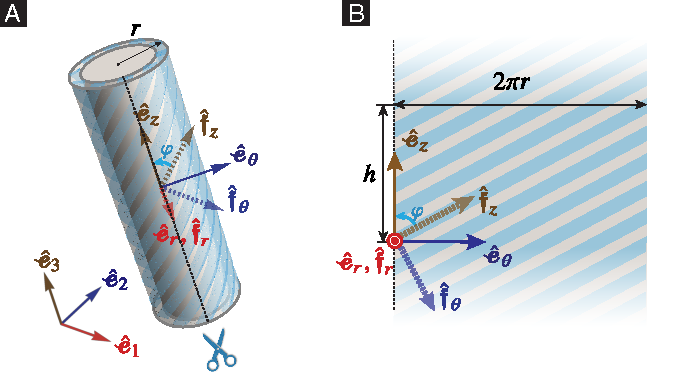
\includegraphics[width=0.8\textwidth]{schematic_V3.pdf}
	\caption{$\subf{A}$ A single-layer cylindrical sturcture with cylindrical orthotropy.~$\subf{B}$ By cutting the hollow cylinder in $\subf{A}$ along the black dashed line, the lateral surface of the cylinder can form a rectanglar sheet of width $2\pi r$.
  }
	\label{fig:schematic}
\end{figure}

%%%%%%%%%%%%%%%%%%%%%%%%%%%%%%%%%%%%%%%%%%%%%%%%%%%%%%%%%%%%%%%%%%%%%%
\subsection{Transformation of constitutive law}
\label{sec:MatrixTrans}
The generalized Hooke's law is
\begin{equation}
\u{\sigma} = \mathbb{C}\, \u{\epsilon},
\label{eq:GeneralizedHooke}
\end{equation}
where~$\u{\sigma}$,~$\u{\epsilon}$, and~$\mathbb{C}$ are the Cauchy stress tensor, infinitesimal strain tensor and elastic stiffness tensor, respectively. Eqn.~\eqref{eq:GeneralizedHooke} can be inverted as

\begin{equation}
 \u{\epsilon} = \mathbb{S}\, \u{\sigma},
\label{eq:GeneralizedHookeInverse}
\end{equation}
where~$\mathbb{S} = \Inv\pr{\mathbb{C}}$ is the elastic compliance tensor, $\Inv\pr{\cdot}$ is the inverse operation.

In the material coordinate system whose basis is~$\pr{\physf_{r}(\theta;\varphi),\physf_{\theta}(\theta;\varphi),\physf_{z}(\theta;\varphi)}$, we rewrite Eqn.~\eqref{eq:GeneralizedHookeInverse} with index notation as
\begin{equation}
\epsilon_{ij}^{\pr{\physf}} = \sum_{k,l \in \mathcal{I}}  S_{ijkl}^{\pr{\physf}} \sigma_{kl}^{\pr{\physf}}, \quad \text{for} \,i,j \in \mathcal{I} ,
\label{eq:GeneralizedHookeComponents}
\end{equation}
where~$\epsilon_{ij}^{\pr{\physf}}$,~$S_{ijkl}^{\pr{\physf}}$, and~$\sigma_{kl}^{\pr{\physf}}$ are the components of~$\u{\sigma}$,~$\mathbb{S}$, and~$\u{\epsilon}$, respectively, with respect to the basis~$\pr{\physf_{r}(\theta;\varphi),\physf_{\theta}(\theta;\varphi),\physf_{z}(\theta;\varphi)}$. For helical fibers with cylindrical orthotropy, the elastic compliance components in its material coordinate system,~$S_{ijkl}^{\pr{\physf}}$, are constant from point to point.
\todo[fancyline]{WF: Need to consider that $\u{\epsilon}$, $\mathbb{S}$, $\u{\sigma}$ are not in the space $\mathbb{E}$. Should introduce more spaces and corresponding bases.}


% In order to express Eqn.~\eqref{eq:GeneralizedHookeComponents} in terms of matrices, we use Voigt notation.
% We introduce elastic compliance matrix~$\usf{S} := \pr{S_{ij}}_{i,j \in\mathcal{I}}$, where~$\mathcal{I} :=\pr{1,\ldots,6}$.
% According to the convention of Voigt notation, the non-zero elements of~$\usf{S}$ are defined as
% \begin{align*}
% & S_{11} := S'_{rrrr},\quad S_{12} := S'_{rr\theta\theta},\quad S_{13} := S'_{rrzz}, \\
% & S_{22} := S'_{\theta\theta\theta\theta},\quad S_{23} := S'_{\theta\theta zz},\quad S_{33} := S'_{zzzz}, \\
% & S_{44} := 2 S'_{\theta z\theta z},\quad S_{55} := 2 S'_{rzrz},\quad S_{66} := 2 S'_{r\theta r\theta}.
% \end{align*}
% We define engineering strain

% Therefore, we express Eqn.~\eqref{eq:GeneralizedHookeComponents} as
% \begin{equation}
% 	\left[
% 		\begin{array}{c}
% 		\epsilon'_{rr} \\ \epsilon'_{\theta\theta} \\ \epsilon'_{zz} \\
% 		2\epsilon'_{\theta z} \\ 2\epsilon'_{r z} \\ 2\epsilon'_{r \theta} \\
% 		\end{array}
% 	\right]
% 	=
% 	\left[
% 		\begin{array}{cccccc}
% 		 S_{11} & S_{12} & S_{13} & 0 & 0 & 0 \\
% 		 S_{12} & S_{22} & S_{23} & 0 & 0 & 0 \\
% 		 S_{13} & S_{23} & S_{33} & 0 & 0 & 0 \\
% 		 0 & 0 & 0 & S_{44} & 0 & 0 \\
% 		 0 & 0 & 0 & 0 & S_{55} & 0 \\
% 		 0 & 0 & 0 & 0 & 0 & S_{66} \\
% 		\end{array}
% 	\right]
% 	\left[
% 		\begin{array}{c}
% 		\sigma'_{rr} \\ \sigma'_{\theta\theta} \\ \sigma'_{zz} \\
% 		\sigma'_{\theta z} \\ \sigma'_{r z} \\ \sigma'_{r \theta} \\
% 		\end{array}
% 	\right],
% \end{equation}

It is desirable to carry out the analysis in the global cylindrical coordinate system of the structure.
Therefore we need to transform the constitutive equation from the material coordinate system to the global cylindrical coordinate system.
As discussed in~$\S$~\ref{sec:bending_model}, The material coordinates are related to the global cylindrical coordinates by a rotation transformation $\usf{Q}(\varphi)$ (see Eqn.~\eqref{eq:Qtransform}). Thus, through change of basis, the compliance form of the generalized Hooke's law in the global cylindrical coordinate system becomes
% \begin{equation}
% 	\left[
% 	\begin{array}{c}
% 	\epsilon_{rr} \\ \epsilon_{\theta\theta} \\ \epsilon_{zz} \\
% 	2\epsilon_{\theta z} \\ 2\epsilon_{r z} \\ 2\epsilon_{r \theta} \\
% 	\end{array}
% 	\right]
% 	=
% 	\left[
% 	\begin{array}{cccccc}
% 	 C_{11} & C_{12} & C_{13} & C_{14} & 0 & 0 \\
% 	 C_{12} & C_{22} & C_{23} & C_{24} & 0 & 0 \\
% 	 C_{13} & C_{23} & C_{33} & C_{34} & 0 & 0 \\
% 	 C_{14} & C_{24} & C_{34} & C_{44} & 0 & 0 \\
% 	 0 & 0 & 0 & 0 & C_{55} & C_{56} \\
% 	 0 & 0 & 0 & 0 & C_{56} & C_{66} \\
% 	\end{array}
% 	\right]
% 	\left[
% 	\begin{array}{c}
% 	\sigma_{rr} \\ \sigma_{\theta\theta} \\ \sigma_{zz} \\
% 	\sigma_{\theta z} \\ \sigma_{rz} \\ \sigma_{r \theta} \\
% 	\end{array}
% 	\right],
% 	\label{eq:HookeGlobal}
% \end{equation}
\begin{equation}
\epsilon_{ij}^{\pr{\physe}} = \sum_{k,l \in \mathcal{I}}  S_{ijkl}^{\pr{\physe}} \sigma_{kl}^{\pr{\physe}}, \quad \text{for} \,i,j \in \mathcal{I} ,
\label{eq:GeneralizedHookeComponentsGlobal}
\end{equation}
where~$\epsilon_{ij}^{\pr{\physe}}$,~$S_{ijkl}^{\pr{\physe}}$, and~$\sigma_{kl}^{\pr{\physe}}$ are the components of~$\u{\sigma}$,~$\mathbb{S}$, and~$\u{\epsilon}$, respectively, with respect to the basis~$(\physe_{r}(\theta),\physe_{\theta}(\theta),\physe_{z}(\theta))$. The relations between two sets of components w.r.t different bases are given by
\begin{align}
\epsilon_{ij}^{\pr{\physe}} & = \sum_{k,l \in \mathcal{I}} Q^{\sf {T}}_{ik} (\varphi) Q^{\sf {T}}_{jl} (\varphi) \epsilon_{kl}^{\pr{\physf}} , \\
\sigma_{ij}^{\pr{\physe}} & = \sum_{k,l \in \mathcal{I}} Q^{\sf {T}}_{ik}(\varphi) Q^{\sf {T}}_{jl}(\varphi) \sigma_{kl}^{\pr{\physf}} , \\
S_{ijkl}^{\pr{\physe}} & = \sum_{p,q,r,s \in \mathcal{I}} Q^{\sf {T}}_{ip}(\varphi) Q^{\sf {T}}_{jq}(\varphi) Q^{\sf {T}}_{kr}(\varphi) Q^{\sf {T}}_{ls}(\varphi) S_{pqrs}^{\pr{\physf}}, \label{eq:SeFromSf}
\end{align}
where $\pr{\cdot}^{\sf {T}}$ is the transpose operation.

Therefore, $S_{ijkl}^{\pr{\physe}}$ can be obtained from $S_{ijkl}^{\pr{\physf}}$ and the helical angle $\varphi$ through relation~\eqref{eq:SeFromSf}.
It should be noted that due to symmetry, the 81 components in neither $S_{ijkl}^{\pr{\physf}}$ nor $S_{ijkl}^{\pr{\physe}}$ are independent.
For a general orthotropic material in its matrial coordinate system, the number of independent compliance constants in~$S_{ijkl}^{\pr{\physf}}$ is nine.
With the addtional variable $\varphi$, there should be ten independent constants in $S_{ijkl}^{\pr{\physe}}$.
% where the transformed elastic compliance matrix~$\pr{C_{ij}}_{i,j \in\mathcal{I}}$, denoted by~$\usf{C}$, should not be confused with the elastic stiffness tensor~$\mathbb{C}$. The relation between~$\usf{C}$ and~$\usf{S}$ is given by
% \begin{subequations}
% \begin{equation}
% \usf{C}= \usf{R}^{-{\sf T}}\usf{S}\usf{R}^{-1},
% \end{equation}
% where
% \begin{equation}
% 	\usf{R}
% 	:=
% 	\left[
% 	\begin{array}{cccccc}
% 	 1 & 0 & 0 & 0 & 0 & 0 \\
% 	 0 & c^2 & s^2 & 2sc & 0 & 0 \\
% 	 0 & s^2 & c^2 & -2sc & 0 & 0 \\
% 	 0 & -sc & sc & c^2 - s^2 & 0 & 0 \\
% 	 0 & 0 & 0 & 0 & c & -s \\
% 	 0 & 0 & 0 & 0 & s & c \\
% 	\end{array}
% 	\right],
% \end{equation}
% \end{subequations}
% with~$s :=\sin \varphi$ and~$c :=\cos \varphi$~\cite{Bower2009}.

% It should be noted that the thirteen non-zero constants~$C_{ij}$ are computed from the nine independent non-zero compliance constants~$S_{ij}$ and the helix angle~$\varphi$. Thus, they are not independent.

%%%%%%%%%%%%%%%%%%%%%%%%%%%%%%%%%%%%%%%%%%%%%%%%%%%%%%%%%%%%%%%%%%%%%%
%\subsection{Governing equations}
%\label{GoverEqs}
%
%In the absence of body force, the elastic equilibrium equation~$\nabla \cdot \boldsymbol{\sigma}=0$ in the cylindrical coordinates has the from
%\begin{equation}
%\begin{aligned}
%& \pd{\sigma_{rr}}{r}+\frac{1}{r}\pd{\tau_{r\theta}}{\theta}+\pd{\tau_{rz}}{z}+\frac{\sigma_{rr} - \sigma_{\theta\theta}}{r} = 0 \\
%& \pd{\tau_{r\theta}}{r}+\frac{1}{r}\pd{\sigma_{\theta\theta}}{\theta}+\pd{\tau_{\theta z}}{z}+\frac{2\sigma_{r\theta}}{r} = 0 \\
%& \pd{\tau_{rz}}{r}+\frac{1}{r}\pd{\tau_{\theta z}}{\theta}+\pd{\sigma_{zz}}{z}+\frac{\sigma_{rz}}{r} = 0 \\
%\end{aligned}
%\end{equation}


%%%%%%%%%%%%%%%%%%%%%%%%%%%%%%%%%%%%%%%%%%%%%%%%%%%%%%%%%%%%%%%%%%%%%%
%\subsection{Verification}
%We first verified the Jolicoeur's results through finite element simulation by comparing the stress components. The radial distribution of~$\sigma_{zz}$ at~$\theta = 90\degree$ in a two-layered curvilinear orthotropic cylinder with helical angle~$\varphi = 15 \degree$ under pure bending is shown in Fig.~\ref{fig:verification}. As we can see, both results are consistent with each other well except very small discrepancy at the interface, which is due to the computation error of contact simulation.
%
%\begin{figure}[t]
%\centering
%\graphicspath{{../LyxFiles/figure/}}
%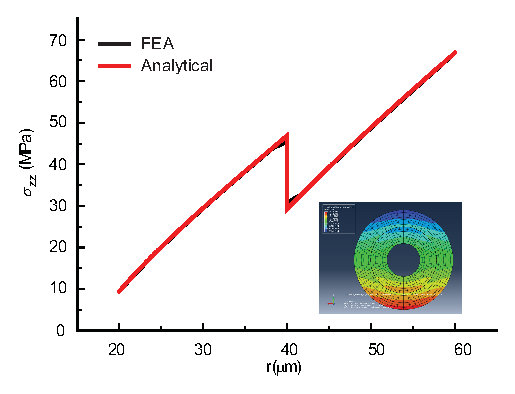
\includegraphics[scale=1]{verification.eps}
%\caption{The radical distribution of~$\sigma_{zz}$ at~$\theta = 90\degree$ of two-layered curvilinear orthotropic cylinder under pure bending computed from finite element analysis and Eqn.XX. Inset: Contour plot of~$\sigma_{zz}$ from finite element simulation.}
%\label{fig:verification}
%\end{figure}


%%%%%%%%%%%%%%%%%%%%%%%%%%%%%%%%%%%%%%%%%%%%%%%%%%%%%%%%%%%%%%%%%%%%%%
\subsection{Bending stiffness formula by Jolicoeur and Cardou}
%The solutions of stresses are
%\begin{equation}
%\begin{aligned}
%\sigma_{rr} & = (\kappa_x \sin\theta - \kappa_y \cos\theta)\left( \sum_{i \in \mathcal{L}} K_i r^{m_i-1} + \mu_1 r \right) \\&+ \sum_{i=1}^{2} K'_i r^{m'_i-1} + \mu_3 \vartheta r + \mu_5 \epsilon \\
%\sigma_{\theta\theta} & = (\kappa_x \sin\theta - \kappa_y \cos\theta)\left( \sum_{i \in \mathcal{L}} K_i (m_i+1) r^{m_i-1} + 3\mu_1 r \right) \\&+ \sum_{i=1}^{2} K'_i m'_i r^{m'_i-1} + 2\mu_3 \vartheta r + \mu_5 \epsilon \\
%\tau_{r\theta} & = (\kappa_x \cos\theta + \kappa_y \sin\theta) \left( -\sum_{i \in \mathcal{L}} K_i r^{m_i-1} - \mu_1 r \right) \\
%\tau_{rz} & = (\kappa_x \cos\theta + \kappa_y \sin\theta) \left( \sum_{i \in \mathcal{L}} K_i g_i r^{m_i-1} + \mu_2 r \right) \\
%\tau_{\theta z} & =  (\kappa_x \sin\theta - \kappa_y \cos\theta)\left( -\sum_{i \in \mathcal{L}} K_i g_i m_i r^{m_i-1} - 2\mu_2 r \right) \\&- \sum_{i=1}^{2} K'_i g'_i r^{m'_i-1} - \mu_4 \vartheta r - \left( \mu_5 \frac{\beta_{14}+\beta_{24}}{\beta_{44}} + \frac{C_{34}}{C_{33}\beta_{44}} \right) \epsilon \\
%\sigma_{zz} & = \frac{1}{C_{33}} \left[ \kappa_x r \sin \theta - \kappa_y r \cos\theta + \epsilon - C_{13} \sigma_r - C_{23} \sigma_{\theta} - C_{34} \tau_{\theta z} \right]
%\end{aligned}
%\end{equation}
\label{sec:bending stiffness}
The bending stiffness of the~$N$-layer cylindrical composite is obtained by Jolicoeur and Cardou as
\begin{equation}
	\begin{aligned}
	EI = & \sum_{n=1}^{N} \left[ \sum_{i \in \mathcal{L}} {}^{n}\!{\alpha_{i}} {}^{n}\!{K_{i}}  \pr{\p\pr{{}^{n-1}\!{r},{}^{n}\!{m_{i}}+2} - \p\pr{{}^{n}\!{r},{}^{n}\!{m_{i}} + 2}} + {}^{n}\!\gamma\pr{\p\pr{{}^{n-1}\!{r},4} - \p\pr{{}^{n}\!{r},4}} \right],
	\end{aligned}
	\label{eq:EI}
\end{equation}
with
\begin{subequations}
	\begin{align}
	{}^{n}\!{\alpha_{i}} & := \frac{\pi}{{}^{n}\!{C_{33}}} \frac{  {}^{n}\!{C_{13}} + {}^{n}\!{C_{23}}({}^{n}\!{m_{i}} + 1) - {}^{n}\!{C_{34}} {}^{n}\!{g_{i}} {}^{n}\!{m_{i}} }{{}^{n}\!{m_{i}}+2}, \\
	{}^{n}\!\gamma & := \frac{\pi}{{}^{n}\!{C_{33}}} \frac{ {}^{n}\!{\mu_{1}} ({}^{n}\!{C_{13}} + 3{}^{n}\!{C_{23}}) - 2{}^{n}\!{\mu_{2}} {}^{n}\!{C_{34}} - 1  }{4},
	\end{align}
\end{subequations}
where~$N$ denotes the total number of layers,~$\mathcal{L} := \pr{1,2,3,4}$,~${}^{n-1}\!{r}$ and~${}^{n}\!{r}$ the internal and external radii of the~$n^\text{th}$ layer,~${}^{n}\!{m_{i}}$,~${}^{n}\!{g_{i}}$,~${}^{n}\!{\mu_{1}}$, and~${}^{n}\!{\mu_{2}}$ are material constants related with elastic constants of the~$n^\text{th}$ layer (see~\ref{Appen:MatConst}). We use $\p\pr{x,y}$ to denote the power operation where $x$ is the base and $y$ is the exponent.

The coefficients~${}^{n}\!{K_{i}}$ are determined by the boundary conditions and continuity conditions of displacement and stress at the interface.

\paragraph{Boundary condition.}

The traction free boundaries at innermost radius~${}^{0}\!{r}$ and outermost radius~${}^{N}\!{r}$ require
\begin{subequations}
	\begin{align}
	\sum_{i \in \mathcal{L}} {}^{1}\!{K_{i}} \p\pr{{}^{0}\!{r},{}^{1}\!{m_{i}} - 2} & = -{}^{1}\!{\mu_{1}}, \quad
	\sum_{i \in \mathcal{L}} {}^{1}\!{K_{i}} {}^{1}\!{g_{i}} \p\pr{{}^{0}\!{r},{}^{1}\!{m_{i}} - 2} = -{}^{1}\!{\mu_{2}},\\
	\sum_{i \in \mathcal{L}} {}^{N}\!{K_{i}} \p\pr{{}^{N}\!{r},{}^{N}\!{m_{i}} - 2} & = -{}^{N}\!{\mu_{1}}, \quad
	\sum_{i \in \mathcal{L}} {}^{N}\!{K_{i}} {}^{N}\!{g_{i}} \p\pr{{}^{N}\!{r},{}^{N}\!{m_{i}} - 2} = -{}^{N}\!{\mu_{2}}.
	\end{align}
	\label{eq:boundary}
\end{subequations}

\paragraph{Interfacial condition: no friction.}

In the case of no friction interface,~$u_r$ and~$\sigma_{rr}$ are continuous,~$\tau_{r\theta}$ and~$\tau_{rz}$ are zero at the interface. Therefore~${}^{n}\!{K_{i}}$ satisfy following equations
\begin{subequations}
	\begin{align}
	\sum_{i \in \mathcal{L}} {}^{n}\!{K_{i}} \p\pr{{}^{n}\!{r},{}^{n}\!{m_{i}} - 2} & = -{}^{n}\!{\mu_{1}}, \quad
	\sum_{i \in \mathcal{L}} {}^{n}\!{K_{i}} {}^{n}\!{g_{i}} \p\pr{{}^{n}\!{r},{}^{n}\!{m_{i}} - 2} = -{}^{n}\!{\mu_{2}}, \\
	\sum_{i \in \mathcal{L}} {}^{n}\!{K_{i}} \p\pr{{}^{n-1}\!{r},{}^{n}\!{m_{i}} - 2} & = -{}^{n}\!{\mu_{1}}, \quad
	\sum_{i \in \mathcal{L}} {}^{n}\!{K_{i}} {}^{n}\!{g_{i}} \p\pr{{}^{n-1}\!{r},{}^{n}\!{m_{i}} - 2} = -{}^{n}\!{\mu_{2}},
	\end{align}
	\label{eq:nofriction_interface}
\end{subequations}
for~$n = 1,2,\dots,N$.


\paragraph{Interfacial condition: no slip.}

In the case of perfect bonding (no slip) interface between layers, the continuity conditions of stresses~$\sigma_{rr}$,~$\tau_{r\theta}$,~$\tau_{rz}$ and displacements~$u_{r}$,~$u_{\theta}$,~$u_z$ at the interface yields
\begin{subequations}
	\begin{align}
	& \sum_{i \in \mathcal{L}} \left( {}^{n}\!{K_{i}} \p\pr{r,{}^{n}\!{m_{i}} - 2} - {}^{n+1}\!{K_{i}} \p\pr{r,{}^{n+1}\!{m_{i}} - 2} \right) = {}^{n+1}\!{\mu_{1}}
  - {}^{n}\!{\mu_{1}}, \\
	& \sum_{i \in \mathcal{L}} \left( {}^{n}\!{K_{i}} {}^{n}\!{g_{i}} \p\pr{r,{}^{n}\!{m_{i}} - 2} - {}^{n+1}\!{K_{i}} {}^{n+1}\!{g_{i}} \p\pr{r,{}^{n+1}\!{m_{i}} - 2} \right) = {}^{n+1}\!{\mu_{2}} - {}^{n}\!{\mu_{2}}, \\
	& \sum_{i \in \mathcal{L}} \left( {}^{n}\!{K_{i}} {}^{n}\!{Q_{i}} \p\pr{r,{}^{n}\!{m_{i}} - 2} - {}^{n+1}\!{K_{i}} {}^{n+1}\!{Q_{i}} \p\pr{r,{}^{n+1}\!{m_{i}} - 2} \right) = {}^{n+1}\!{Q_{5}} - {}^{n}\!{Q_{5}}, \\
	& \sum_{i \in \mathcal{L}} \left( {}^{n}\!{K_{i}} {}^{n}\!{W_{i}} \p\pr{r,{}^{n}\!{m_{i}} - 2} - {}^{n+1}\!{K_{i}} {}^{n+1}\!{W_{i}} \p\pr{r,{}^{n+1}\!{m_{i}} - 2} \right) = {}^{n+1}\!{W_{5}} - {}^{n}\!{W_{5}},
	\end{align}
	\label{eq:noslip_interface}
\end{subequations}
for~$n = 1,2,\dots,N-1$, where~$Q_i$ and~$W_i$ ($i=$1 to 5) are material constants (see~\ref{Appen:MatConst}).





%%%%%%%%%%%%%%%%%%%%%%%%%%%%%%%%%%%%%%%%%%%%%%%%%%%%%%%%%%%%%%%%%%%%%%
\section{Effective bending stiffness}
\label{sec:limit_analysis}
In this section, we derive the asymptotic bending stiffness of multilayer cylindrical structure.
Specifically, for a given lamination scheme, we analyze the asymptotic behavior of Eqn.~\eqref{eq:EI} by limiting the total number of layers,~$N$, to infinity.
The asymptotic expansion is performed under the following assumptions: (i) We assume that the cross-section area of the structure is constant and the thickness of each layer is equal and vanishing as~$N$ goes to infinity. (ii) We also assume that the constitutive properties of all layers are the same in their own material coordinate system. But the principal material property orientations, i.e. helical angles, of the layers may be different.

We use the stacking-sequence notation to describe the spatial arrangement of layers' helical angles. As per stacking-sequence notation, we use~$[{}^{0}\!\varphi]_N$ to denote a lamination scheme consisting of~$N$ layers and all layers have same helical angle,~${}^{0}\!\varphi$. 
For this lamination scheme, the material property of a material point does not change with its position in the cylinder. Thus the material is essentially homogeneous.
It should be noted that even though all layers share the same helical angle, the pitch sizes $p$ of different layers may not be the same. According to the relation $\tan{({}^{0}\!\varphi)} = p/(2\pi r )$, for inner layer with smaller radius than that of the outer layer, the pitch size is smaller.


We also consider cases where the helical angles are not uniform and the composed material becomes heterogeneous. We use~$[{}^{I}\!\varphi/{}^{II}\!\varphi]_{N/2}$ to denote a lamination scheme consisting of~$N$ layers where layers with helical angles~${}^{I}\!\varphi$ and~${}^{II}\!\varphi$ are alternatively arranged. 

Based on the lamination schemes and interfacial conditions, we consider three different scenarios here. (i) Homogeneous material-No friction: the lamination scheme is~$[{}^{0}\!\varphi]_N$ and no friction exists between layers. (ii) Heterogeneous material-No friction: the lamination scheme is~$[{}^{I}\!\varphi/{}^{II}\!\varphi]_{N/2}$ and the interfaces between layers is frictionless. (iii) Heterogeneous material-No slip: the lamination scheme is~$[{}^{I}\!\varphi/{}^{II}\!\varphi]_{N/2}$ as well, but there is no slip between the interfaces.

%%%%%%%%%%%%%%%%%%%%%%%%%%%%%%%%%%%%%%%%%%%%%%%%%%%%%%%%%%%%%%%%%%%%%%
\subsection{Homogeneous material and no friction interface}
\label{sec:1mat_no_friction}

First we consider that the elastic property for each layer is the same. The interfaces between layers are frictionless. This is equivalent to the scenario where a homogeneous cylinder is cut into layers with uniform thickness and there is no friction between the layers. In this case, we drop the subscript~$n$ of the material constants for the sake of simplicity. To obtain the coefficients~${}^{n}\!{K_{i}}$, we rewrite Eqns.~\eqref{eq:boundary} and~\eqref{eq:nofriction_interface} as
\begin{equation}
	\begin{bmatrix}
	\p\pr{{}^{n}\!{r},m_1 - 2} & \p\pr{{}^{n}\!{r},m_2 - 2} & \p\pr{{}^{n}\!{r},m_3 - 2} & \p\pr{{}^{n}\!{r},m_4 - 2} \\
	g_1 \p\pr{{}^{n}\!{r},m_1 - 2} & g_2 \p\pr{{}^{n}\!{r},m_2 - 2} & g_3 \p\pr{{}^{n}\!{r},m_3 - 2} & g_4 \p\pr{{}^{n}\!{r},m_4 - 2} \\
	\p\pr{{}^{n-1}\!{r},m_1 - 2} & \p\pr{{}^{n-1}\!{r},m_2 - 2} & \p\pr{{}^{n-1}\!{r},m_3 - 2} & \p\pr{{}^{n-1}\!{r},m_4 - 2} \\
	g_1 \p\pr{{}^{n-1}\!{r},m_1 - 2} & g_2 \p\pr{{}^{n-1}\!{r},m_2 - 2} & g_3 \p\pr{{}^{n-1}\!{r},m_3 - 2} & g_4 \p\pr{{}^{n-1}\!{r},m_4 - 2}
	\end{bmatrix}
	\begin{bmatrix}
	{}^{n}\!{K_{1}} \\ {}^{n}\!{K_{2}} \\ {}^{n}\!{K_{3}} \\ {}^{n}\!{K_{4}}
	\end{bmatrix}
	=
	\begin{bmatrix}
	-\mu_1 \\ -\mu_2 \\ -\mu_1 \\ -\mu_2
	\end{bmatrix},
	\label{eq:eqs of Kin_one_mat_no_friction}
\end{equation}
for~$n = 1,2,\dots,N$. Let layer thickness~$\Delta r := \pr{{}^{N}\!{r}-{}^{0}\!{r}}/N$, radius sequence~${}^{n}\!{r} := {}^{0}\!{r} + n\cdot \Delta r$. Applying Taylor series expansion on the inverse of the coefficient matrix of~${}^{n}\!{K_{i}}$ around~${}^{n}\!{r}$, we have
\begin{equation}
	{}^{n}\!{K_{i}} = P_i \cdot \p\pr{{}^{n}\!{r},-m_i  + 2} + O(\Delta r), \quad \text{for}\, i \in \mathcal{L},
	\label{eq:single_mat_Ks}
\end{equation}
where~$P_i$ are material constants given in~\ref{Appen:Pi}. Substituting Eqn.~\eqref{eq:single_mat_Ks} into Eqn.~\eqref{eq:EI}, we have
\begin{equation}
	\begin{aligned}
	EI & = \sum_{n=1}^{N} \left[ \sum_{i \in \mathcal{L}} \alpha_i \left( P_i \p\pr{{}^{n}\!{r},-m_i  + 2} + O(\Delta r) \right) \pr{\p\pr{{}^{n-1}\!{r},{}^{n}\!{m_{i}} + 2} - \p\pr{{}^{n}\!{r},m_{i} +2}} \right] + \gamma \pr{\p\pr{{}^{0}\!{r},4} - \p\pr{{}^{N}\!{r},4}} \\
	 & \begin{split}
		= \sum_{n=1}^{N} \left[ \sum_{i \in \mathcal{L}} \alpha_i \left( P_i \p\pr{{}^{n}\!{r},-m_i  + 2} + O(\Delta r) \right) (- \p\pr{{}^{n}\!{r},m_{i} +1}(m_i + 2 ) \Delta r + O(\p\pr{\Delta r,2})) \right] \\
		+ \gamma \pr{\p\pr{{}^{0}\!{r},4} - \p\pr{{}^{N}\!{r},4}}
	   \end{split}\\
	 & = - \sum_{n=1}^{N} \left[ \sum_{i \in \mathcal{L}} \left( \alpha_i P_i (m_i + 2 ) \p\pr{{}^{n}\!{r},3} \cdot \Delta r \right) \right] + \gamma \pr{\p\pr{{}^{0}\!{r},4} - \p\pr{{}^{N}\!{r},4}} + O\pr{\p\pr{\Delta r,2}}.
	\end{aligned}
	\label{eq:single_mat_EI}
\end{equation}
Taking the limit~$N \to \infty$, according to the definition of Riemann integral, we convert the sum of series in Eqn.~\eqref{eq:single_mat_EI} into integral to derive the asymptotic bending stiffness as
\begin{equation}
	\begin{aligned}
	(EI)_{\infty} & = - \lim\limits_{N \to \infty} \sum_{n=1}^{N} \left[ \sum_{i \in \mathcal{L}} \alpha_i P_i (m_i + 2 ) \p\pr{{}^{n}\!{r},3} \Delta r \right] + \gamma \pr{\p\pr{{}^{0}\!{r},4} - \p\pr{{}^{N}\!{r},4}} + O\pr{\p\pr{\Delta r,2}} \\
	 & = - \sum_{i \in \mathcal{L}} \left( \int_{{}^{0}\!{r}}^{{}^{N}\!{r}} \alpha_i P_i (m_i + 2 ) \p\pr{r,3} \, dr \right) + \gamma \pr{\p\pr{{}^{0}\!{r},4} - \p\pr{{}^{N}\!{r},4}} \\
	 & = - \frac{\p\pr{{}^{N}\!{r},4} - \p\pr{{}^{0}\!{r},4}}{4} \left[ \sum_{i \in \mathcal{L}} \alpha_i P_i (m_i + 2 ) + 4\gamma\right].
	\end{aligned}
	\label{eq:single_mat_EI_final}
\end{equation}



%%%%%%%%%%%%%%%%%%%%%%%%%%%%%%%%%%%%%%%%%%%%%%%%%%%%%%%%%%%%%%%%%%%%%%
\subsection{Heterogeneous material and no friction interface}
\label{sec:2mat_no_friction}
We consider the lamination scheme of the multilayered cylindrical composite as~$[{}^{I}\!\varphi/{}^{II}\!\varphi]_{N/2}$. That is, layers with helical angles~${}^{I}\!\varphi$ and~${}^{II}\!\varphi$ are alternatively arranged from the core to the periphery of the cylinder. We use~$I$ and~$II$ as subscripts to denote material constants of layers with odd and even layer numbers.
Under no friction interfacial condition~\eqref{eq:nofriction_interface} and considering boundary condition~\eqref{eq:boundary}, the~${}^{n}\!{K_{i}}$ can be solved from the following equations
\begin{equation}
	\begin{bmatrix}
		\p\pr{{}^{n}\!{r},{}^{n}\!{m_{1}} - 2} & \p\pr{{}^{n}\!{r},{}^{n}\!{m_{2}} - 2} & \p\pr{{}^{n}\!{r},{}^{n}\!{m_{3}} - 2} & \p\pr{{}^{n}\!{r},{}^{n}\!{m_{4}} - 2} \\
		{}^{n}\!{g_{1}} \p\pr{{}^{n}\!{r},{}^{n}\!{m_{1}} - 2} & {}^{n}\!{g_{2}} \p\pr{{}^{n}\!{r},{}^{n}\!{m_{2}} - 2} & {}^{n}\!{g_{3}} \p\pr{{}^{n}\!{r},{}^{n}\!{m_{3}} - 2} & {}^{n}\!{g_{4}} \p\pr{{}^{n}\!{r},{}^{n}\!{m_{4}} - 2} \\
		\p\pr{{}^{n-1}\!{r},{}^{n}\!{m_{1}} - 2} & \p\pr{{}^{n-1}\!{r},{}^{n}\!{m_{2}} - 2} & \p\pr{{}^{n-1}\!{r},{}^{n}\!{m_{3}} - 2} & \p\pr{{}^{n-1}\!{r},{}^{n}\!{m_{4}} - 2} \\
		{}^{n}\!{g_{1}} \p\pr{{}^{n-1}\!{r},{}^{n}\!{m_{1}} - 2} & {}^{n}\!{g_{2}} \p\pr{{}^{n-1}\!{r},{}^{n}\!{m_{2}} - 2} & {}^{n}\!{g_{3}} \p\pr{{}^{n-1}\!{r},{}^{n}\!{m_{3}} - 2} & {}^{n}\!{g_{4}} \p\pr{{}^{n-1}\!{r},{}^{n}\!{m_{4}} - 2}
	\end{bmatrix}
	\begin{bmatrix}
		{}^{n}\!{K_{1}} \\ {}^{n}\!{K_{2}} \\ {}^{n}\!{K_{3}} \\ {}^{n}\!{K_{4}}
	\end{bmatrix}
	=
	\begin{bmatrix}
		-{}^{n}\!{\mu_{1}} \\ -{}^{n}\!{\mu_{2}} \\ -{}^{n}\!{\mu_{1}} \\ -{}^{n}\!{\mu_{2}}
	\end{bmatrix},
	\label{eq:eqs of Kin_two_mat_no_friction}
\end{equation}
for~$n = 1,2,\dots,N$. In this case,~${}^{n}\!{K_{i}}$ of adjacent layers are not coupled with each other and thus can be obtained by using the similar technique being used in the homogeneous material case. Applying Taylor series expansion on the inverse of the coefficient matrix of~${}^{n}\!{K_{i}}$ around~${}^{n}\!{r}$ gives
\begin{equation}
	{}^{n}\!{K_{i}} = {}^{n}\!{P_{i}} \cdot \p\pr{{}^{n}\!{r},-{}^{n}\!{m_{i}} + 2} + O(\Delta r), \quad \text{for}\, i \in \mathcal{L},
	\label{eq:two_mat_no_friction_Ks}
\end{equation}
where~${}^{n}\!{P_{i}}$ are material constants of the~$n^{\text{th}}$ layer (see~\ref{Appen:Pi}).  Substituting Eqn.~\eqref{eq:two_mat_no_friction_Ks} into Eqn.~\eqref{eq:EI}, we have
\begin{equation}
	\begin{aligned}
	\begin{split}
	EI & = \sum_{n=1}^{N} \bigg[ \sum_{i \in \mathcal{L}} {}^{n}\!{\alpha_{i}} \left( {}^{n}\!{P_{i}} \p\pr{{}^{n}\!{r},-{}^{n}\!{m_{i}} + 2} + O(\Delta r) \right) \cdot \\ & \qquad{} (- \p\pr{{}^{n}\!{r},{}^{n}\!{m_{i}}+1}({}^{n}\!{m_{i}} + 2 ) \Delta r + O(\p\pr{\Delta r,2}))  + {}^{n}\!\gamma (-4 \p\pr{{}^{n}\!{r},3} \Delta r + O(\p\pr{\Delta r,2})) \bigg] \\
	 & = -\sum_{n=1}^{N} \bigg[ \sum_{i \in \mathcal{L}} {}^{n}\!{\alpha_{i}} {}^{n}\!{P_{i}} ({}^{n}\!{m_{i}} + 2) + 4{}^{n}\!\gamma \bigg] \p\pr{{}^{n}\!{r},3} \cdot \Delta r + O(\p\pr{\Delta r,2}).
	\end{split}
	\end{aligned}
	\label{eq:two_mat_no_friction_EI_1}
\end{equation}
Since the arrangement of material property is periodic, the odd layers share the same material constants~${}^{I}\!{\alpha_{i}}$,~${}^{I}\!{P_{i}}$,~${}^{I}\!{m_{i}}$, and~${}^{I}\!\gamma$ while the even layers share the same material constants~${}^{II}\!{\alpha_{i}}$,~${}^{II}\!{P_{i}}$,~${}^{II}\!{m_{i}}$, and~${}^{II}\!\gamma$. We rewrite Eqn.~\eqref{eq:two_mat_no_friction_EI_1} as
\begin{equation}
	\begin{aligned}
		EI & = -\sum_{\text{odd layers}} \bigg[ \sum_{i \in \mathcal{L}} {}^{I}\!{\alpha_{i}} {}^{I}\!{P_{i}} ({}^{I}\!{m_{i}} + 2) + 4{}^{I}\!\gamma \bigg] \p\pr{{}^{n}\!{r},3} \cdot \Delta r \\ & \quad{} -\sum_{\text{even layers}} \bigg[ \sum_{i \in \mathcal{L}} {}^{II}\!{\alpha_{i}} {}^{II}\!{P_{i}} ({}^{II}\!{m_{i}} + 2) + 4{}^{II}\!\gamma \bigg] \p\pr{{}^{n}\!{r},3} \cdot \Delta r + O(\p\pr{\Delta r,2}) \\
		 & = -\frac{1}{2}
		 \bigg\lbrace
		 \sum_{n=1}^N \bigg[ \sum_{i \in \mathcal{L}} {}^{I}\!{\alpha_{i}} {}^{I}\!{P_{i}} ({}^{I}\!{m_{i}} + 2) + 4{}^{I}\!\gamma \bigg] \p\pr{{}^{n}\!{r},3} \cdot \Delta r \\ & \quad\qquad{} + \sum_{n=1}^N \bigg[ \sum_{i \in \mathcal{L}} {}^{II}\!{\alpha_{i}} {}^{II}\!{P_{i}} ({}^{II}\!{m_{i}} + 2) + 4{}^{II}\!\gamma \bigg] \p\pr{{}^{n}\!{r},3} \cdot \Delta r
		 \bigg\rbrace + O(\p\pr{\Delta r,2}).
	\end{aligned}
	\label{eq:two_mat_no_friction_EI_2}
\end{equation}
Taking the limit~$N \to \infty$, according to the definition of Riemann integral, the Eqn.~\eqref{eq:two_mat_no_friction_EI_2} becomes
\begin{equation}
	 \begin{aligned}
	   (EI)_{\infty} & = \frac{1}{2}  \Biggl \{
	   		- \Biggl[ \sum_{i \in \mathcal{L}} {}^{I}\!{\alpha_{i}} {}^{I}\!{P_{i}} ({}^{I}\!{m_{i}} + 2) + 4{}^{I}\!\gamma \Biggr]
			\int_{{}^{0}\!{r}}^{{}^{N}\!{r}} \p\pr{r,3} \, dr \\ & \quad\qquad{}
			- \Biggl[ \sum_{i \in \mathcal{L}} {}^{II}\!{\alpha_{i}} {}^{II}\!{P_{i}} ({}^{II}\!{m_{i}} + 2) + 4{}^{II}\!\gamma \Biggr]
			\int_{{}^{0}\!{r}}^{{}^{N}\!{r}} \p\pr{r,3} \, dr
	    \Biggl \} \\
	    & = \frac{1}{2} \left[ {}^{I}(EI)_{\infty} + {}^{II}(EI)_{\infty} \right],
	 \end{aligned}
	\label{eq:two_mat_no_friction_EI}
\end{equation}
where
\begin{equation}
	{}^{j}(EI)_{\infty} = - \frac{\p\pr{{}^{N}\!{r},4} - \p\pr{{}^{0}\!{r},4}}{4} \left[ \sum_{i \in \mathcal{L}} {}^{j}\!{\alpha_{i}} {}^{j}\!{P_{i}} ({}^{j}\!{m_{i}} + 2 ) + 4{}^{j}\!\gamma\right], \quad \text{for} \, j = I, II.
\end{equation}


%%%%%%%%%%%%%%%%%%%%%%%%%%%%%%%%%%%%%%%%%%%%%%%%%%%%%%%%%%%%%%%%%%%%%%
\subsection{Heterogeneous material and no slip interface}
\label{sec:2mat_no_slip}
For the case that the lamination scheme of the multilayered cylindrical composite is~$[{}^{I}\!\varphi/{}^{II}\!\varphi]_{N/2}$ under no slip interfacial condition, the~$4N$ unknowns~${}^{n}\!{K_{i}}$ can be solved from the boundary conditions by Eqn.~\eqref{eq:boundary} and the interfacial conditions by Eqn.~\eqref{eq:noslip_interface}, which can be rewritten as
\begin{equation}
\begin{aligned}
& \begin{bmatrix}
	\p\pr{{}^{n-1}\!{r},{}^{n-1}\!{m_{1}}} & \p\pr{{}^{n-1}\!{r},{}^{n-1}\!{m_{2}}} & \p\pr{{}^{n-1}\!{r},{}^{n-1}\!{m_{3}}} & \p\pr{{}^{n-1}\!{r},{}^{n-1}\!{m_{4}}} \\
	{}^{n-1}\!{g_{1}} \p\pr{{}^{n-1}\!{r},{}^{n-1}\!{m_{1}}} & {}^{n-1}\!{g_{2}} \p\pr{{}^{n-1}\!{r},{}^{n-1}\!{m_{2}}} & {}^{n-1}\!{g_{3}} \p\pr{{}^{n-1}\!{r},{}^{n-1}\!{m_{3}}} & {}^{n-1}\!{g_{4}} \p\pr{{}^{n-1}\!{r},{}^{n-1}\!{m_{4}}} \\
	{}^{n-1}\!{Q_{1}} \p\pr{{}^{n-1}\!{r},{}^{n-1}\!{m_{1}}} & {}^{n-1}\!{Q_{2}} \p\pr{{}^{n-1}\!{r},{}^{n-1}\!{m_{2}}} & {}^{n-1}\!{Q_{3}} \p\pr{{}^{n-1}\!{r},{}^{n-1}\!{m_{3}}} & {}^{n-1}\!{Q_{4}} \p\pr{{}^{n-1}\!{r},{}^{n-1}\!{m_{4}}} \\
	{}^{n-1}\!{W_{1}} \p\pr{{}^{n-1}\!{r},{}^{n-1}\!{m_{1}}} & {}^{n-1}\!{W_{2}} \p\pr{{}^{n-1}\!{r},{}^{n-1}\!{m_{2}}} & {}^{n-1}\!{W_{3}} \p\pr{{}^{n-1}\!{r},{}^{n-1}\!{m_{3}}} & {}^{n-1}\!{W_{4}} \p\pr{{}^{n-1}\!{r},{}^{n-1}\!{m_{4}}}
\end{bmatrix}
\begin{bmatrix}
	{}^{n-1}\!{K_{1}} \\ {}^{n-1}\!{K_{2}} \\ {}^{n-1}\!{K_{3}} \\ {}^{n-1}\!{K_{4}}
\end{bmatrix}\\
& =
  \begin{bmatrix}
	\p\pr{{}^{n-1}\!{r},{}^{n}\!{m_{1}}} & \p\pr{{}^{n-1}\!{r},{}^{n}\!{m_{2}}} & \p\pr{{}^{n-1}\!{r},{}^{n}\!{m_{3}}} & \p\pr{{}^{n-1}\!{r},{}^{n}\!{m_{4}}} \\
	{}^{n}\!{g_{1}} \p\pr{{}^{n-1}\!{r},{}^{n}\!{m_{1}}} & {}^{n}\!{g_{2}} \p\pr{{}^{n-1}\!{r},{}^{n}\!{m_{2}}} & {}^{n}\!{g_{3}} \p\pr{{}^{n-1}\!{r},{}^{n}\!{m_{3}}} & {}^{n}\!{g_{4}} \p\pr{{}^{n-1}\!{r},{}^{n}\!{m_{4}}} \\
	{}^{n}\!{Q_{1}} \p\pr{{}^{n-1}\!{r},{}^{n}\!{m_{1}}} & {}^{n}\!{Q_{2}} \p\pr{{}^{n-1}\!{r},{}^{n}\!{m_{2}}} & {}^{n}\!{Q_{3}} \p\pr{{}^{n-1}\!{r},{}^{n}\!{m_{3}}} & {}^{n}\!{Q_{4}} \p\pr{{}^{n-1}\!{r},{}^{n}\!{m_{4}}} \\
	{}^{n}\!{W_{1}} \p\pr{{}^{n-1}\!{r},{}^{n}\!{m_{1}}} & {}^{n}\!{W_{2}} \p\pr{{}^{n-1}\!{r},{}^{n}\!{m_{2}}} & {}^{n}\!{W_{3}} \p\pr{{}^{n-1}\!{r},{}^{n}\!{m_{3}}} & {}^{n}\!{W_{4}} \p\pr{{}^{n-1}\!{r},{}^{n}\!{m_{4}}}
  \end{bmatrix}
  \begin{bmatrix}
	{}^{n}\!{K_{1}} \\ {}^{n}\!{K_{2}} \\ {}^{n}\!{K_{3}} \\ {}^{n}\!{K_{4}}
  \end{bmatrix}
-
\begin{bmatrix}
	{}^{n}\!{D_{1}} \\ {}^{n}\!{D_{2}} \\ {}^{n}\!{D_{3}} \\ {}^{n}\!{D_{4}}
\end{bmatrix},
\label{eq:eqs of Kin_two_mat_no_slip_original}
\end{aligned}
\end{equation}
for~$n = 2,3,\dots,N$, where
\begin{equation}
	\begin{bmatrix}
		{}^{n}\!{D_{1}} \\ {}^{n}\!{D_{2}} \\ {}^{n}\!{D_{3}} \\ {}^{n}\!{D_{4}}
	\end{bmatrix}
	= - \p\pr{{}^{n-1}\!{r},2}
	\begin{bmatrix}
		{}^{n}\!{\mu_{1}}-{}^{n-1}\!{\mu_{1}} \\ {}^{n}\!{\mu_{2}}-{}^{n-1}\!{\mu_{2}}  \\ {}^{n}\!{Q_{5}}-{}^{n-1}\!{Q_{5}} \\ {}^{n}\!{W_{5}}-{}^{n-1}\!{W_{5}}
	\end{bmatrix}.
\end{equation}

Using bold san-serif font symbol to denote matrices, we rewrite Eqn.~\eqref{eq:eqs of Kin_two_mat_no_slip_original} as
\begin{equation}
	~^{n}{\usf{B}} ~^{n-1}{\usf{K}} = ~^{n}{\usf{A}} ~^{n}{\usf{K}} - ~^{n}{\usf{D}},
	\label{eq:eqs of Kin_two_mat_no_slip_np1}
\end{equation}
for~$n = 2,3,\dots,N$. The matrices~$~^{{n-1}}{\usf{K}}$ and~$~^{n}{\usf{K}}$ are coupled with each other in this case. Therefore, each~$~^{n}{\usf{K}}$ cannot be solved individually.

We come up with a differential equation based asymptotic analysis method to estimate~$~^{n}{\usf{K}}$ as~$N$ approaches infinity. For the sake of clarity, we only post essential steps of the derivation in this section. For the details of the complete derivation, we ask the readers to refer to~\ref{Appen:derivations}.

We first substitute~$n$ as~$n-1$ into Eqn.~\eqref{eq:eqs of Kin_two_mat_no_slip_np1} and combine the resulting equation with Eqn.~\eqref{eq:eqs of Kin_two_mat_no_slip_np1} to find out the relation between~$~^{n}{\usf{K}}$ and~$~^{{n-2}}{\usf{K}}$ as
\begin{equation}
	~^{n}{\usf{A}} ~^{n}{\usf{K}}  = ~^{n}{\usf{B}} \Inv\pr{{}^{{n-1}}\usf{A}} ~^{{n-1}}{\usf{B}} ~^{{n-2}}{\usf{K}} + ~^{n}{\usf{B}} \Inv\pr{{}^{{n-1}}\usf{A}} ~^{{n-1}}{\usf{D}}  + ~^{n}{\usf{D}} .
	\label{eq:knknm2}
\end{equation}
In Eqn.~\eqref{eq:knknm2}, we take Taylor series expansion on~$\Inv\pr{{}^{{n-1}}\usf{A}}$ and~$~^{{n-1}}{\usf{B}}$ around~${}^{n-1}\!{r}$ to obtain (see~\ref{Appen:Eqn315} for details)
\begin{subequations}
	\begin{align}
	& ~^{n}{\usf{B}} \Inv\pr{{}^{{n-1}}\usf{A}} ~^{{n-1}}{\usf{B}} = ~^{n}{\usf{A}} + \frac{\Delta r}{~^{n-1}\!{r}} \left( ~^{n}{\usf{B}} ~^{n-1}\tilde{\usf{m}} \Inv\pr{{}^{n}\usf{B}} ~^{n}{\usf{A}} - ~^{n}{\usf{A}} ~^{n}\tilde{\usf{m}} \right)  + O(\p\pr{\Delta r,2}), \\
	& ~^{n}{\usf{B}} \Inv\pr{{}^{{n-1}}\usf{A}} ~^{{n-1}}{\usf{D}} + ~^{n}{\usf{D}} = \frac{\Delta r}{~^{n-1}\!{r}} \left( 2~^{n}{\usf{D}} + ~^{n}{\usf{B}} ~^{n-1}\tilde{\usf{m}} \Inv\pr{{}^{n}\usf{B}} ~^{{n-1}}{\usf{D}} \right) + O(\p\pr{\Delta r,2}),
	\end{align}
	\label{eq:bnanm1}
\end{subequations}
Then by substituting Eqn.~\eqref{eq:bnanm1} into Eqn.~\eqref{eq:knknm2}, we obtain
\begin{equation}
\begin{aligned}
	\begin{split}
	~^{n}{\usf{A}} ~^{n}{\usf{K}} & = \left[  ~^{n}{\usf{A}} + \frac{\Delta r}{~^{n-1}\!{r}} \left( ~^{n}{\usf{B}} ~^{n-1}\tilde{\usf{m}} \Inv\pr{{}^{n}\usf{B}} ~^{n}{\usf{A}} - ~^{n}{\usf{A}} ~^{n}\tilde{\usf{m}} \right)  + O(\p\pr{\Delta r,2}) \right] ~^{{n-2}}{\usf{K}} \\
	& \qquad + \frac{\Delta r}{~^{n-1}\!{r}} \left( 2~^{n}{\usf{D}} + ~^{n}{\usf{B}} ~^{n-1}\tilde{\usf{m}} \Inv\pr{{}^{n}\usf{B}} ~^{{n-1}}{\usf{D}} \right) + O(\p\pr{\Delta r,2}),
	\end{split}
\end{aligned}
\label{eq:knknm2appr1}
\end{equation}
which gives the asymptotic relation between~$~^{{n-2}}{\usf{K}}$ and~$~^{n}{\usf{K}}$.
From a set of representative plots for~$K_{i}$ versus~$n$ of a 100-layered structure (see Fig.~\ref{fig:two_material_no_slip_Ks}), we deduce that the~$K_{i}$ of odd (and even) layer numbers are continuous in the asymptotic sense (for~$N \to \infty$), which are indicated by red dashed lines. Hence, we approximate~$~^{{n-2}}{\usf{K}}$ to the first order of~$\Delta r$ as
\begin{equation}
	~^{{n-2}}{\usf{K}} = ~^{n}{\usf{K}} - 2\frac{d~^{n}{\usf{K}}}{dr} \Delta r + O(\p\pr{\Delta r,2}).
	\label{eq:knknm2appr2}
\end{equation}
\begin{figure}[t]
	\centering
	\graphicspath{{../LyxFiles/figure/}}
	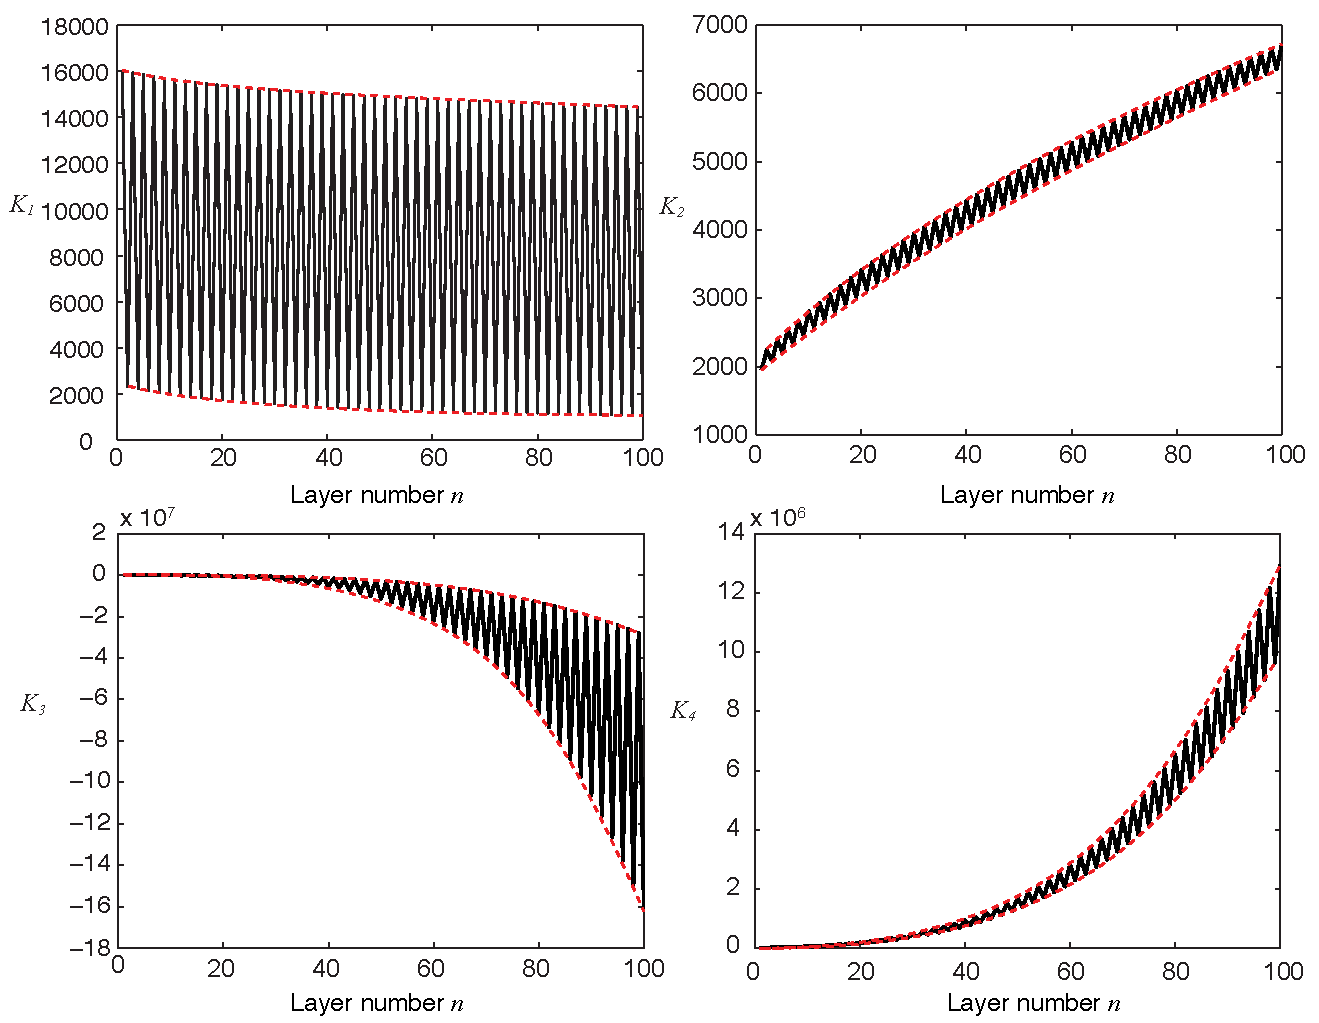
\includegraphics[width=1\textwidth]{two_material_no_slip_Ks.pdf}
	\caption{A set of representative plots of~$K_i$ with layer number~$n$ for a cylindrical composite with lamination scheme~$[-15 \degree/25 \degree]_{50}$ under no slip interfacial condition.}
	\label{fig:two_material_no_slip_Ks}
\end{figure}

Substituting Eqn.~\eqref{eq:knknm2appr2} into Eqn.~\eqref{eq:knknm2appr1} and making simplification (see~\ref{Appen:GovernEqnKn} for details), we obtain a linear ordinary differential equation (ODE) system of~$~^{n}{\usf{K}}$
\begin{equation}
  2 ~^{n}\!{r} \frac{d \pr{~^{n}\usf{f}({}^{n}\!r)~^{n}{\usf{K}}}}{dr} = \pr{~^{n}\tilde{\usf{M}} + ~^{n}\tilde{\usf{m}}} \pr{~^{n}\usf{f}({}^{n}\!r){}^{n}{\usf{K}}} + \p\pr{{}^{n}\!{r},2} ~^{n}\tilde{\usf{F}},
	\label{eq:GovernEqnKn}
\end{equation}
with boundary conditions given by Eqn.~\eqref{eq:boundary}. Solving this linear ODE system (see~\ref{Appen:SolvingODE} for the details of the solution procedures), we obtain
\begin{equation}
%{}^{n}\!{K_{i}} = {}^{n}\!{r}^{-{}^{n}\!{m_{i}}} \left( {}^{n}\!G_{i0} \p\pr{{}^{n}\!{r},2} + G^1_{i,n} r^{{}^{n}\!{\lambda_{1}}}_n + G^2_{i,n} r^{{}^{n}\!{\lambda_{2}}}_n + G^3_{i,n} r^{{}^{n}\!{\lambda_{3}}}_n + G^4_{i,n} r^{{}^{n}\!{\lambda_{4}}}_n \right)
{}^{n}\!{K_{i}} = \p\pr{{}^{n}\!{r},-{}^{n}\!{m_{i}}} \left( {}^{n}\!G_{i0} \p\pr{{}^{n}\!{r},2} + \sum_{j \in \mathcal{L}} {}^{n}\!G_{ij} \p\pr{{}^{n}\!{r},{}^{n}\!\lambda_{j}} \right), \quad \text{for}\, i \in \mathcal{L},
\label{eq:two_mat_no_slip_Ks}
\end{equation}
where~${}^{n}\!G_{ij}$ ($j = \text{0 to 4}$) and~${}^{n}\!\lambda_{j}$ ($j \in \mathcal{L}$) given by Eqn.~\eqref{eq:Gjin} are constants related to material constants of the~$n^{\text{th}}$ layer.
Substituting Eqn.~\eqref{eq:two_mat_no_slip_Ks} into Eqn.~\eqref{eq:EI}, we obtain the bending stiffness as
\begin{equation}
\begin{aligned}
	EI & = - \sum_{n=1}^{N} \left\lbrace \sum_{i \in \mathcal{L}} {}^{n}\!{\hat{\alpha}_{i}} \left( {}^{n}\!G_{i0} \p\pr{{}^{n}\!{r},2} + \sum_{j \in \mathcal{L}} {}^{n}\!G_{ij} \p\pr{{}^{n}\!{r},{}^{n}\!\lambda_{j}} \right) {}^{n}\!{r} + 4{}^{n}\!\gamma~ \p\pr{{}^{n}\!{r},3} \right\rbrace + O(\Delta r) \\
	& =  - \sum_{n=1}^{N} \left\lbrace \left( \sum_{i \in \mathcal{L}} {}^{n}\!{\hat{\alpha}_{i}} {}^{n}\!G_{i0} + 4{}^{n}\!\gamma \right) \p\pr{{}^{n}\!{r},3}+ \sum_{i \in \mathcal{L}} \sum_{j \in \mathcal{L}} {}^{n}\!{\hat{\alpha}_{i}} {}^{n}\!G_{ij} \p\pr{{}^{n}\!{r},1 + {}^{n}\!\lambda_{j}} \right\rbrace + O(\Delta r),
\end{aligned}
\end{equation}
where~${}^{n}\!{\hat{\alpha}_{i}} := {}^{n}\!{\alpha_{i}} \left( {}^{n}\!{m_{i}} + 2\right)$.

Since the material properties of the layers of the structure are alternately arranged, the odd layers share the same material constants~${}^{I}\!{\alpha_{i}}$,~${}^{I}\!\gamma$,~${}^{I}\!{m_{i}}$,~${}^{I}\!G_{ij}$, and~${}^{I}\!\lambda_{j}$, and the even layers have the same constants~${}^{II}\!{\alpha_{i}}$,~${}^{II}\!\gamma$,~${}^{II}\!{m_{i}}$,~${}^{II}\!G_{ij}$, and~${}^{II}\!\lambda_{j}$. Therefore,
\begin{equation}
\begin{aligned}
	EI & =  - \frac{1}{2} \sum_{n=1}^{N} \left[ \left( \sum_{i \in \mathcal{L}} {}^{I}\!\hat{\alpha}_{i} {}^{I}\!G_{i0} + 4{}^{I}\!\gamma \right) \p\pr{{}^{n}\!{r},3}+ \sum_{i \in \mathcal{L}} \sum_{j \in \mathcal{L}} {}^{I}\!\hat{\alpha}_{i} {}^{I}\!G_{ij} \p\pr{{}^{n}\!{r},1 + {}^{I}\!\lambda_{j}} \right] \\
	 & \quad - \frac{1}{2} \sum_{n=1}^{N} \biggr[ \left( \sum_{i \in \mathcal{L}} {}^{II}\!\hat{\alpha}_{i} {}^{II}\!G_{i0} + 4{}^{II}\!\gamma \right) \p\pr{{}^{n}\!{r},3} \\
	  & \qquad \qquad \qquad \qquad + \sum_{i \in \mathcal{L}} \sum_{j \in \mathcal{L}} {}^{II}\!\hat{\alpha}_{i} {}^{II}\!G_{ij} \p\pr{{}^{n}\!{r},1 + {}^{II}\!\lambda_{j}} \biggr] + O(\Delta r).
\end{aligned}
\end{equation}
As~$N \to \infty$, we obtain the asymptotic bending stiffness as
\begin{equation}
\begin{aligned}
	(EI)_{\infty} & =  - \frac{1}{2} \left[ \sum_{i \in \mathcal{L}} \left( {}^{I}\!\hat{\alpha}_{i} {}^{I}\!G_{i0} + {}^{II}\!\hat{\alpha}_{i} {}^{II}\!G_{i0} \right) + 4\left( {}^{I}\!\gamma +{}^{II}\!\gamma \right) \right] \int_{{}^{0}\!{r}}^{{}^{N}\!{r}} \p\pr{r,3} \, dr \\
	& \quad - \frac{1}{2} \sum_{i \in \mathcal{L}} \sum_{j \in \mathcal{L}} \left[ \int_{{}^{0}\!{r}}^{{}^{N}\!{r}} \left( {}^{I}\!\hat{\alpha}_{i} {}^{I}\!G_{ij} \p\pr{r,1 + {}^{I}\!\lambda_{j}} + {}^{II}\!\hat{\alpha}_{i} {}^{II}\!G_{ij}  \p\pr{r,1 + {}^{II}\!\lambda_{j}} \right) \, dr \right] \\
	& = - \frac{1}{8} \left[ \sum_{i \in \mathcal{L}} \left( {}^{I}\!\hat{\alpha}_{i} {}^{I}\!G_{i0} + {}^{II}\!\hat{\alpha}_{i} {}^{II}\!G_{i0} \right) + 4\left( {}^{I}\!\gamma +{}^{II}\!\gamma \right) \right] \left( \p\pr{{}^{N}\!{r},4} - \p\pr{{}^{0}\!{r},4} \right) \\
	& \quad - \frac{1}{2} \sum_{i \in \mathcal{L}} \sum_{j \in \mathcal{L}} \biggr[ \frac{{}^{I}\!\hat{\alpha}_{i} {}^{I}\!G_{ij}}{2 + {}^{I}\!\lambda_{j} } \left( \p\pr{{}^{N}\!{r},2 + {}^{I}\!\lambda_{j}} - \p\pr{{}^{0}\!{r},2 + {}^{I}\!\lambda_{j}} \right) \\
	& \qquad \qquad \qquad \quad + \frac{{}^{II}\!\hat{\alpha}_{i} {}^{II}\!G_{ij}}{2 + {}^{II}\!\lambda_{j}} \left( \p\pr{{}^{N}\!{r},2 + {}^{II}\!\lambda_{j}} - \p\pr{{}^{0}\!{r},2 + {}^{II}\!\lambda_{j}} \right) \biggr] .
\end{aligned}
\label{eq:two_mat_no_slip_EI}
\end{equation}

%%%%%%%%%%%%%%%%%%%%%%%%%%%%%%%%%%%%%%%%%%%%%%%%%%%%%%%%%%%%%%%%%%%%%%
\section{Numerical examples and discussions}
\label{sec:discussion}
In this section, the bending stiffness of multilayered cylindrical structures with different lamination schemes and interfacial conditions are numerical studied and the asymptotic bending stiffness derived in~$\S$\ref{sec:limit_analysis} are validated.

The the cylindrical composite is divided into~$N$ co-axial layers with constant thickness.
The innermost and outermost radii of the cylindrical structure are taken to be~${}^{0}\!{r} = 2$ mm and~${}^{N}\!{r} = 14$ mm, respectively.
Three different combinations of lamination schemes and interfacial conditions are considered: (i)~$[-15 \degree]_N$ and~$[25 \degree]_N$ with no friction interfacial condition, (ii)~$[-15 \degree/ 25 \degree]_{N/2}$ with no friction interfacial condition, (iii)~$[-15 \degree/25 \degree]_{N/2}$ with no slip interfacial condition. In all three scenarios, the non-zero elastic compliance components of cylindrically orthotropic material in each layer's in material coordinate system are the same and provided in Tab.~\ref{tab:sij}.
\begin{table}[h]
  \begin{center}
    \caption{Elastic compliance components of cylindrically orthotropic material in material coordinate system ($10^{-10}$ m$^2$/N) }
    \label{tab:sij}
    \begin{tabular}{|c|c|c|c|c|c|c|c|c|}\hline
      $S_{11}$ & $S_{12}$ & $S_{13}$ & $S_{22}$ & $S_{23}$ &
      $S_{33}$ & $S_{44}$ & $S_{55}$ & $S_{66}$  \\ \hline
      1.05 & -0.0632 & -0.0842 & 1.18 & -0.0941 &
      0.20 & 4.00 & 5.00 & 2.50  \\ \hline
    \end{tabular}
  \end{center}
\end{table}

The relation between bending stiffness and total layer number~$N$ for the structure consisting of homogeneous material with no friction interface is shown as solid line in Fig.~\ref{fig:asymptotic_EI}~$\subf{A}$. The bending stiffnesses of one-layer cylinders are 881.47 N$\cdot$m$^2$ and 528.11 N$\cdot$m$^2$ for the materials with -15$\degree$ and 25$\degree$ helical angles, respectively.
As we increase the total layer number, for both materials, the bending stiffness first decreases rapidly then becomes stable after~$N$ is greater than five. Although the layer thickness approaches to zero as~$N \to \infty$, the bending stiffness converges to a non-zero constant, which is given by Eqn.~\eqref{eq:single_mat_EI_final}. The asymptotic bending stiffness of composite with lamination scheme~$[-15 \degree]_{\infty}$ and~$[25 \degree]_{\infty}$ are 722.15 N$\cdot$m$^2$ and 412.13 N$\cdot$m$^2$, respectively (see Fig.~\ref{fig:asymptotic_EI}~$\subf{A}$).
%\begin{figure}[h]
%	\centering
%	\graphicspath{{../LyxFiles/figure/}}
%	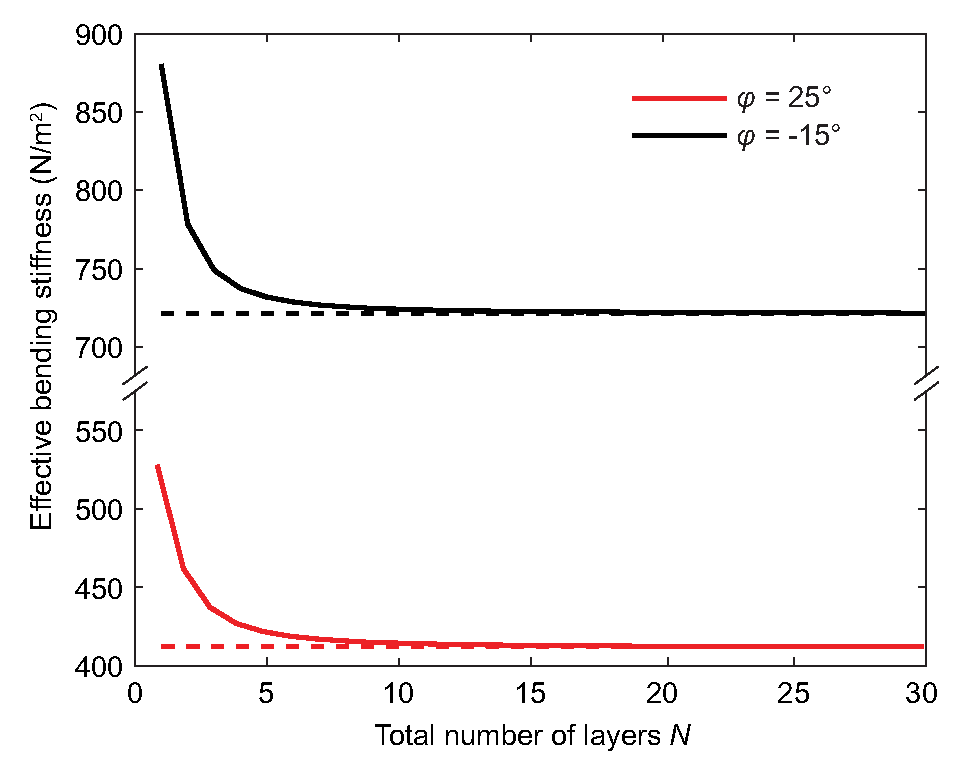
\includegraphics[width=0.8\textwidth]{single_material_EI.eps}
%	\caption{The change of effective bending stiffness with total number of layers (solid line) and the asymptotic bending stiffness for infinite layers (dashed line) of homogeneous material under no friction interfacial condition.}
%	\label{fig:single_material_EI}
%\end{figure}

The relation between bending stiffness and total layer number for the heterogeneous layer properties with no friction interface is plotted as solid line in Fig.~\ref{fig:asymptotic_EI}~$\subf{B}$.
The lamination scheme for this case is~$[-15 \degree/ 25 \degree]_{N/2}$. The bending stiffness oscillates as the total layer number increases due to the alternated arrangement of the layer properties. Eventually, it approaches to a non-zero constant as~$N \to \infty$, which is the asymptotic bending stiffness given by Eqn.~\eqref{eq:two_mat_no_friction_EI}. The asymptotic homogenized bending stiffness of the heterogeneous structure is 567.14 N$\cdot$m$^2$ (see Fig.~\ref{fig:asymptotic_EI}~$\subf{B}$), which is equal to the average of those of two homogeneous materials.
%\begin{figure}[h]
%	\centering
%	\graphicspath{{../LyxFiles/figure/}}
%	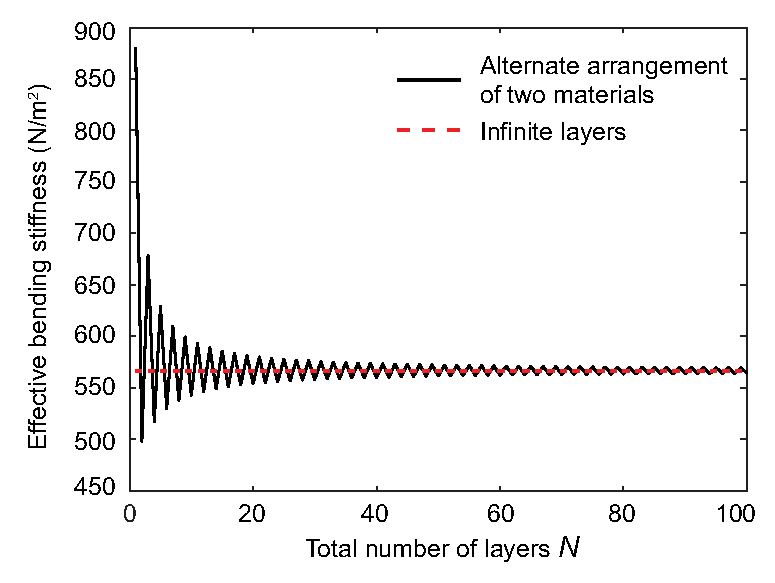
\includegraphics[width=0.8\textwidth]{two_material_no_friction_EI.eps}
%	\caption{The change of bending stiffness with total number of layers (solid line) and the asymptotic bending stiffness for infinite layers (dashed line) of two materials with periodic arrangement under no friction interfacial condition.}
%	\label{fig:two_material_no_friction_EI}
%\end{figure}

The plot of bending stiffness with total layer number for the heterogeneous material and no slip interface case, in which the lamination scheme is~$[-15 \degree/ 25 \degree]_{N/2}$, is shown as solid line in Fig.~\ref{fig:asymptotic_EI}~$\subf{C}$. The bending stiffness oscillates as the total layer number increases and approaches to a non-zero constant, which is the asymptotic bending stiffness given by Eqn.~\eqref{eq:two_mat_no_slip_EI}. Furthermore, it is interesting to note that the asymptotic bending stiffness of heterogeneous structures exceeds the bending stiffness of both homogeneous structures.
The maximum bending stiffness, 1093.12 N$\cdot$m$^2$, is achieved when the total layer number is five.
The asymptotic bending stiffness, 1046.94 N$\cdot$m$^2$, is higher than those of the structures consisting of homogeneous materials, which are 881.47 N$\cdot$m$^2$ and 528.11 N$\cdot$m$^2$. This implies that we could build up stiffer composite from compliant materials by designing the spatial arrangements of laminae.
%\begin{figure}[t]
%	\centering
%	\graphicspath{{../LyxFiles/figure/}}
%	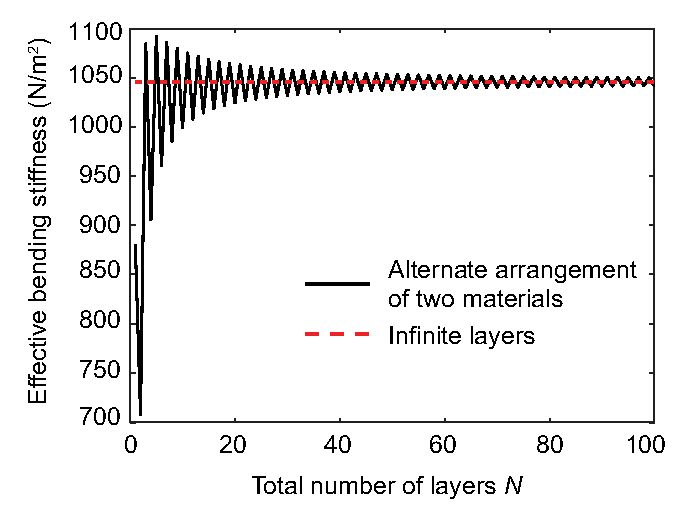
\includegraphics[width=0.8\textwidth]{two_material_no_slip_EI.eps}
%	\caption{The change of bending stiffness with total number of layers (solid line) and the asymptotic bending stiffness for infinite layers (dashed line) of two materials with periodic arrangement under no slip interfacial condition.}
%	\label{fig:two_material_no_slip_EI}
%\end{figure}

The enhancement effect in bending stiffness of the heterogeneous structures with no slip interface also sheds light on the role of multilayered cylindrical orthotropic structures as observed in a number of structural biomaterials.
We believe this kind of internal structure is designed to enhance the effective bending stiffness of the biomaterials to support external loads. To see this, we also numerically studied the bending stiffness of the structure made up with isotropic materials. However we found that there is no enhancement in the asymptotic bending stiffness when the alternative layers are made of isotropic materials. The difference of cylindrical orthotropic and isotropic material lies in the constitutive equations. For the cylindrical orthotropic material, the elastic constants~$C_{i4}$ ($i \in \mathcal{L}$) is non-zero, which implies that the axis stress~$\sigma_{zz}$ and shear strain~$\epsilon_{\theta z}$ are coupled.

\begin{figure}[h!]
	\centering
	\graphicspath{{../LyxFiles/figure/}}
	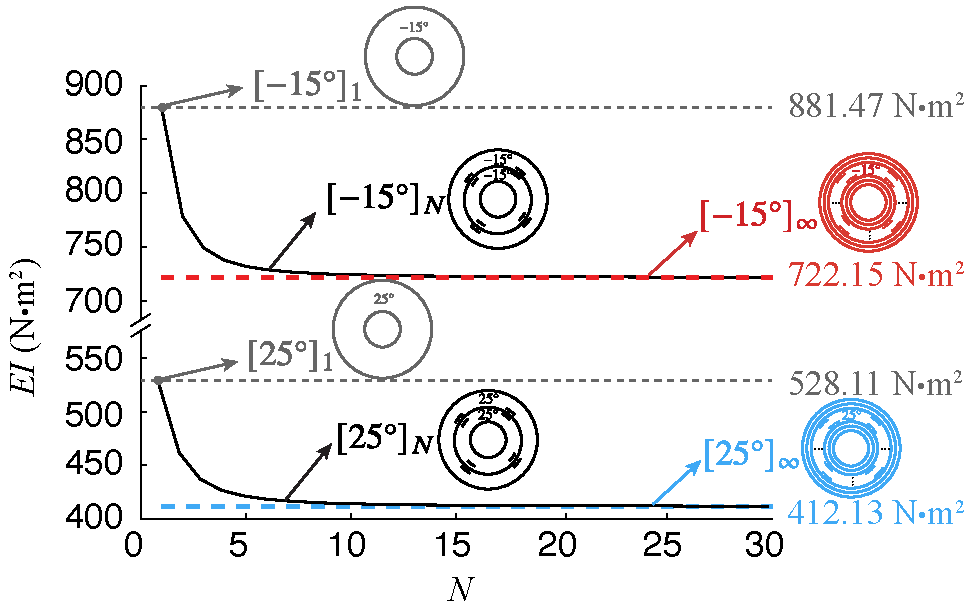
\includegraphics[width=0.6\textwidth]{NoFractionHomo_V2.pdf}
	\caption{The variations of effective bending stiffness as the number of layers increases (solid lines) and their asymptotic limits as the number of layers approach infinity (dashed lines) under different combinations of lamination schemes and interfacial properties:~$\subf{A}$~$[-15 \degree]_N$ and~$[25 \degree]_N$ with no friction interfacial condition,~$\subf{B}$~$[-15 \degree/ 25 \degree]_{N/2}$ with no friction interfacial condition,~$\subf{C}$~$[-15 \degree/25 \degree]_{N/2}$ with no slip interfacial condition.}
	\label{fig:asymptotic_EI}
\end{figure}

\begin{figure}[h!]
  \centering
  \graphicspath{{../LyxFiles/figure/}}
  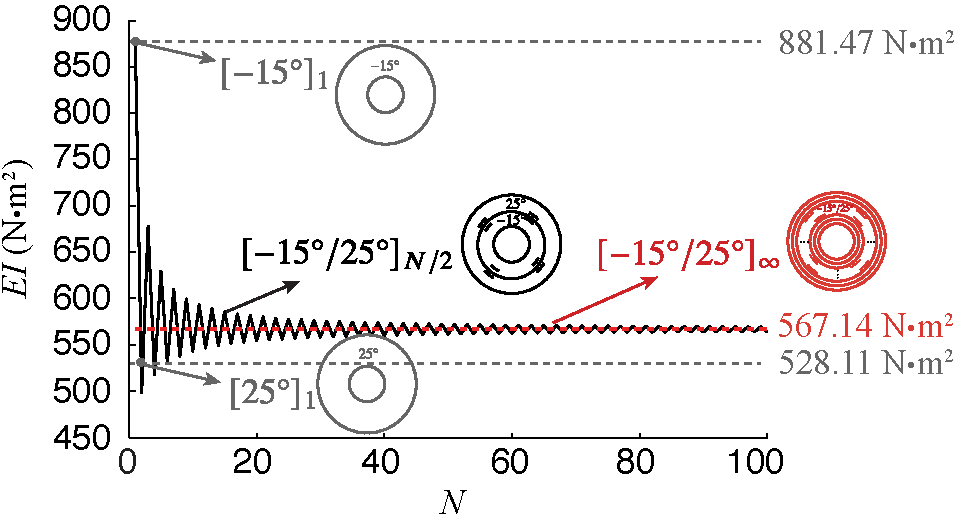
\includegraphics[width=0.6\textwidth]{NoFractionHete_V2.pdf}
  \caption{The variations of effective bending stiffness as the number of layers increases (solid lines) and their asymptotic limits as the number of layers approach infinity (dashed lines) under different combinations of lamination schemes and interfacial properties:~$\subf{A}$~$[-15 \degree]_N$ and~$[25 \degree]_N$ with no friction interfacial condition,~$\subf{B}$~$[-15 \degree/ 25 \degree]_{N/2}$ with no friction interfacial condition,~$\subf{C}$~$[-15 \degree/25 \degree]_{N/2}$ with no slip interfacial condition.}
  \label{fig:asymptotic_EI}
\end{figure}

\begin{figure}[h!]
  \centering
  \graphicspath{{../LyxFiles/figure/}}
  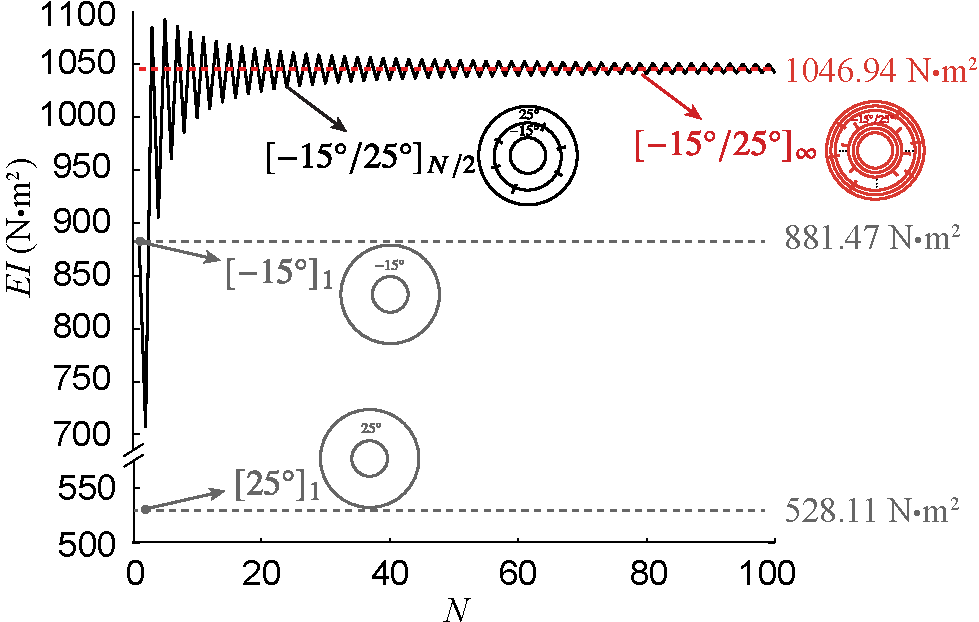
\includegraphics[width=0.6\textwidth]{NoSlipHete_V2.pdf}
  \caption{The variations of effective bending stiffness as the number of layers increases (solid lines) and their asymptotic limits as the number of layers approach infinity (dashed lines) under different combinations of lamination schemes and interfacial properties:~$\subf{A}$~$[-15 \degree]_N$ and~$[25 \degree]_N$ with no friction interfacial condition,~$\subf{B}$~$[-15 \degree/ 25 \degree]_{N/2}$ with no friction interfacial condition,~$\subf{C}$~$[-15 \degree/25 \degree]_{N/2}$ with no slip interfacial condition.}
  \label{fig:asymptotic_EI}
\end{figure}
%%%%%%%%%%%%%%%%%%%%%%%%%%%%%%%%%%%%%%%%%%%%%%%%%%%%%%%%%%%%%%%%%%%%%%
\section{Conclusions}
\label{sec:conclusion}
In order to obtain the asymptotic bending stiffness of multilayered composite cylindrical structures with curvilinear orthotropy, we present a asymptotic analysis of bending stiffness by considering infinite number of layers in this paper.
Analytical expressions of asymptotic bending stiffness are obtained by considering the no slip and no friction interfacial conditions and geometric arrangement of layers with different material properties.
Although we only consider two materials properties for the heterogeneous structure, we believe that the method used in this work can be extended to multiple materials properties with similar analysis procedures.
We show that it is possible to create stiffer structures from compliant materials by appropriate geometric arrangement, which provide guidance in creating bio-inspired materials with desirable mechanical properties.


%%%%%%%%%%%%%%%%%%%%%%%%%%%%%%%%%%%%%%%%%%%%%%%%%%%%%%%%%%%%%%%%%%%%%%
\section*{Acknowledgements}
%Financial support from XX is appreciated.
W.L. Deng acknowledges the graduate fellowship from the China Scholarship Council.


%% The Appendices part is started with the command \appendix;
%% appendix sections are then done as normal sections
\newpage
\appendix

\section{Material constants}
\label{Appen:MatConst}
The material constants~$m_i$,~$g_i$,~$Q_i$,~$W_i$ and~$\mu_i$ are dependent on elastic constants.
We calculate~$m_i$ as
\begin{subequations}
	\begin{align}
	 m_1 & =  \sqrt{\frac{-b +\sqrt{\p\pr{b,2} - 4ac}}{2a}}, \\
	 m_2 & =  \sqrt{\frac{-b -\sqrt{\p\pr{b,2} - 4ac}}{2a}}, \\
	 m_3 & =  -\sqrt{\frac{-b +\sqrt{\p\pr{b,2} - 4ac}}{2a}}, \\
	 m_4 & =  -\sqrt{\frac{-b -\sqrt{\p\pr{b,2} - 4ac}}{2a}}, \\
	\intertext{where}
	 a & :=  \beta_{22} \beta_{44} - \p\pr{\beta_{24},2}, \\
	\begin{split}
	 b & := \beta_{24}(2\beta_{14} + \beta_{24} + 2\beta_{56}) + \p\pr{\beta_{14},2} \\
	 & \quad - \beta_{44}(\beta_{11} + 2\beta_{12} + \beta_{22} + \beta_{66}) - \beta_{22} \beta_{55},
	\end{split} \\
	c & :=  \beta_{55}(\beta_{11} + 2\beta_{12} + \beta_{22} + \beta_{66})-\p\pr{\beta_{56},2},
	\end{align}
\end{subequations}
and the reduced elastic constants~$\beta_{ij}$ are defined in terms of~$C_{ij}$ as
\begin{equation}
\beta_{ij} := C_{ij}-\frac{C_{i3} C_{3j}}{C_{33}}.
\end{equation}


We calculate~$g_i$,~$Q_i$,~$W_i$ as
\begin{subequations}
	\begin{align}
	g_i & = \frac{\beta_{24}\p\pr{m_i,2}+(\beta_{14} + \beta_{24})m_i - \beta_{56}}{\beta_{44}\p\pr{m_i,2} - \beta_{55}}, \\
	Q_i & = \frac{1}{m_i} \pr{\beta_{12}m_i + \beta_{22}m_i(m_i+1) - \beta_{24} g_i \p\pr{m_i,2}}, \\
	W_i & = \frac{1}{m_i}\pr{\beta_{55} g_i - \beta_{56}},
	\end{align}
\end{subequations}
for~$ i \in \mathcal{L}$.

We calculate~$Q_5$ and~$W_5$ as
\begin{subequations}
	\begin{align}
	Q_5 & = \mu_1(\beta_{12} + 3\beta_{22})-2\mu_2\beta_{24} + \frac{C_{23}}{C_{33}}, \\
	W_5 & = \frac{1}{2}(\beta_{55}\mu_2 - \beta_{56}\mu_1),
	\end{align}
	where
	\begin{equation}
	\begin{bmatrix}
		\mu_1 \\ \mu_2
	\end{bmatrix} :=
	\frac{1}{C_{33}}
	\Inv \pr{\begin{bmatrix}
		-2\beta_{14}-6\beta_{24}+\beta_{56} & 4\beta_{44}-\beta_{55} \\
		-\beta_{11}-2\beta_{12}+3\beta_{22}-\beta_{66} & 2\beta_{14}-2\beta_{24}+\beta_{56}
	\end{bmatrix}}
	\begin{bmatrix}
			2C_{34} \\ C_{13}-C_{23}
	\end{bmatrix}.
	\end{equation}
\end{subequations}


\section{Expressions of~$P_i$}
\label{Appen:Pi}
The expressions of~$P_i$ in Eqn.~\eqref{eq:single_mat_Ks} are given by
\begin{subequations}
\begin{align}
	\begin{split}
	P_1 & = -\frac{1}{p} \left(\left(g_2 g_3 (m_2 - m_3)(m_4 -2) + g_2 g_4 (m_4 - m_2)(m_3 - 2) \right.\right.\\
	&\qquad{} \left. + g_3 g_4 (m_3 - m_4)(m_2 -2) \right) \mu_1  + \left(g_2 (m_3 - m_4)(m_2 -2) \right. \\
	&\qquad{} \left.\left. + g_3(m_4 - m_2)(m_3 -2) + g_4 (m_2 - m_3)(m_4 -2) \right)\mu_2 \right) ,
	\end{split} \\
	\begin{split}
	P_2 & = \frac{1}{p} \left(\left( g_1 g_3 (m_1 - m_3)(m_4 -2) + g_1 g_4 (m_4 - m_1)(m_3 - 2)\right.\right. \\
	&\qquad{} \left. + g_3 g_4 (m_3 - m_4)(m_1 -2)  \right) \mu_1 + \left(g_1 (m_3 - m_4)(m_1 -2) \right.\\
	&\qquad{} \left.\left. + g_3(m_4 - m_1)(m_3 -2) + g_4 (m_1 - m_3)(m_4 -2)  \right)\mu_2  \right),
	\end{split} \\
	\begin{split}
	P_3 & = -\frac{1}{p} ((g_1 g_2 (m_1 - m_2)(m_4 -2) + g_1 g_4 (m_4 - m_1)(m_2 - 2) \\ &\qquad{} + g_2 g_4 (m_2 - m_4)(m_1 -2) ) \mu_1 + (g_1 (m_2 - m_4)(m_1 -2) \\  &\qquad{} + g_2(m_4 - m_1)(m_2 -2) + g_4 (m_1 - m_2)(m_4 -2))\mu_2),
	\end{split} \\
	\begin{split}
	P_4 & = \frac{1}{p} ((g_1 g_2 (m_1 - m_2)(m_3 -2) + g_1 g_3 (m_3 - m_1)(m_2 - 2) \\ &\qquad{} + g_2 g_3 (m_2 - m_3)(m_1 -2)) \mu_1 +  (g_1 (m_2 - m_3)(m_1 -2) \\  &\qquad{} + g_2(m_3 - m_1)(m_2 -2) + g_3 (m_1 - m_2)(m_3 -2))\mu_2),
	\end{split}
	\end{align}
\end{subequations}
where
\begin{equation}
	\begin{aligned}
	p := & g_1(g_3 - g_4)(m_1 - m_3)(m_2 - m_4) \\
	 	& + g_2(g_3 - g_4)(m_2 - m_3)(m_4 - m_1) \\
	 	& - (g_1 g_2 + g_3 g_4 - g_1 g_4 - g_2 g_4)(m_1 - m_2)(m_3 - m_4).
	\end{aligned}
\end{equation}

\section{Derivations in~$\S$\ref{sec:2mat_no_slip}}
\label{Appen:derivations}
\subsection{Derivations of Eqn.~\eqref{eq:bnanm1}}
\label{Appen:Eqn315}
To obtain Eqn.~\eqref{eq:bnanm1}, let
\begin{subequations}
\begin{align}
	~^{n}\tilde{\usf{A}}
	& :=
	\begin{bmatrix}
		1 & 1 & 1 & 1 \\
		{}^{n}\!{g_{1}} & {}^{n}\!{g_{2}} & {}^{n}\!{g_{3}} & {}^{n}\!{g_{4}} \\
		{}^{n}\!{Q_{1}} & {}^{n}\!{Q_{2}} & {}^{n}\!{Q_{3}} & {}^{n}\!{Q_{4}} \\
		{}^{n}\!{W_{1}} & {}^{n}\!{W_{2}} & {}^{n}\!{W_{3}} & {}^{n}\!{W_{4}}
	\end{bmatrix}, \\
	~^{n}\tilde{\usf{B}}
	& :=
	\begin{bmatrix}
		1 & 1 & 1 & 1 \\
		{}^{n-1}\!{g_{1}} & {}^{n-1}\!{g_{2}} & {}^{n-1}\!{g_{3}} & {}^{n-1}\!{g_{4}} \\
		{}^{n-1}\!{Q_{1}} & {}^{n-1}\!{Q_{2}} & {}^{n-1}\!{Q_{3}} & {}^{n-1}\!{Q_{4}} \\
		{}^{n-1}\!{W_{1}} & {}^{n-1}\!{W_{2}} & {}^{n-1}\!{W_{3}} & {}^{n-1}\!{W_{4}}
	\end{bmatrix}, \\
	~^{n}\usf{f}(r)
	& :=
	\begin{bmatrix}
		\p\pr{r,{}^{n}\!{m_{1}}} & 0 & 0 & 0 \\
		0 & \p\pr{r,{}^{n}\!{m_{2}}} & 0 & 0 \\
		0 & 0 & \p\pr{r,{}^{n}\!{m_{3}}} & 0 \\
		0 & 0 & 0 & \p\pr{r,{}^{n}\!{m_{4}}}
	\end{bmatrix}, \\
	~^{n}\tilde{\usf{m}}
	& :=
	\begin{bmatrix}
		{}^{n}\!{m_{1}} & 0 & 0 & 0 \\
		0 & {}^{n}\!{m_{2}} & 0 & 0 \\
		0 & 0 & {}^{n}\!{m_{3}} & 0 \\
		0 & 0 & 0 & {}^{n}\!{m_{4}}
	\end{bmatrix}.
	\end{align}
	\label{eq:C1}
\end{subequations}
It is noted that~$~^{n}\tilde{\usf{A}}$,~$~^{n}\tilde{\usf{B}}$, and~$~^{n}\tilde{\usf{m}}$ are constant matrices. The coefficient matrices~${}^{n}{\usf{A}}$ and~$~^{n}{\usf{B}}$ in Eqn.~\eqref{eq:eqs of Kin_two_mat_no_slip_original} can be written as
\begin{equation}
	~^{n}{\usf{A}} = ~^{n}\tilde{\usf{A}}  ~^{n}\usf{f}({}^{n-1}\!r), \quad
	~^{n}{\usf{B}} = ~^{n}\tilde{\usf{B}}  ~^{n-1}\usf{f}({}^{n-1}\!r).
\end{equation}
Approximating~$~^{{n-1}}{\usf{A}}$ and~$~^{{n-1}}{\usf{B}}$ to the first order of~$\Delta r$ around~${}^{n-1}\!{r}$, we have
\begin{subequations}
\begin{align}
	~^{{n-1}}{\usf{A}} & = ~^{n}\usf{B} - \delta ~^{n}\usf{B} \Delta r + O(\p\pr{\Delta r,2}), \\
	~^{{n-1}}{\usf{B}} & = ~^{n}\usf{A} - \delta ~^{n}\usf{A} \Delta r + O(\p\pr{\Delta r,2}),
\end{align}
\end{subequations}
where
\begin{subequations}
	\begin{align}
	\delta ~^{n}\usf{A} & = \frac{1}{~^{n-1}\!{r}} ~^{n}\usf{A} ~^{n}\tilde{\usf{m}} = \frac{1}{~^{n-1}\!{r}} ~^{n}\tilde{\usf{A}} ~^{n}\usf{f}({}^{n-1}\!r) ~^{n}\tilde{\usf{m}}, \\
	\delta ~^{n}\usf{B} & = \frac{1}{~^{n-1}\!{r}} ~^{n}\usf{B} ~^{n-1}\tilde{\usf{m}} = \frac{1}{~^{n-1}\!{r}} ~^{n}\tilde{\usf{B}} ~^{n-1}\usf{f}({}^{n-1}\!r) ~^{n-1}\tilde{\usf{m}}.
	\end{align}
\end{subequations}
Therefore,
\begin{subequations}
	\begin{align}
	\begin{split}
		~^{n}{\usf{B}} \Inv\pr{{}^{{n-1}}\usf{A}}
		& = ~^{n}{\usf{B}} \Inv\left[ ~^{n}\usf{B} - \delta ~^{n}\usf{B} \Delta r + O(\p\pr{\Delta r,2}) \right] \\
		& = ~^{n}{\usf{B}} \Inv\left[ ~^{n}\usf{B} \left( \usf{I}_{4\times 4}- \frac{\Delta r}{~^{n-1}\!{r}} ~^{n-1}\tilde{\usf{m}} \right) + O(\p\pr{\Delta r,2}) \right] \\
		& = ~^{n}{\usf{B}} \Inv\left[ \usf{I}_{4\times 4} - \frac{\Delta r}{~^{n-1}\!{r}} ~^{n-1}\tilde{\usf{m}} + O(\p\pr{\Delta r,2}) \right] \Inv\pr{{}^{{n}}\usf{B}} \\
		& = \usf{I}_{4\times 4} + \frac{\Delta r}{~^{n-1}\!{r}} ~^{n}{\usf{B}}\  ~^{n-1}\tilde{\usf{m}}\  \Inv\pr{{}^{n}\usf{B}} + O(\p\pr{\Delta r,2}),
	\end{split}\\
	\begin{split}
		~^{n}{\usf{B}} \Inv\pr{{}^{{n-1}}\usf{A}} ~^{{n-1}}{\usf{B}}
		& = \left[ \usf{I}_{4\times 4} + \frac{\Delta r}{~^{n-1}\!{r}} ~^{n}{\usf{B}} ~^{n-1}\tilde{\usf{m}} \Inv\pr{{}^{n}\usf{B}} + O(\p\pr{\Delta r,2}) \right] \cdot \\
		& \qquad \left[ ~^{n}\usf{A} - \frac{\Delta r}{~^{n-1}\!{r}} ~^{n}{\usf{A}} ~^{n}\tilde{\usf{m}} + O(\p\pr{\Delta r,2}) \right] \\
		& = ~^{n}\usf{A} + \frac{\Delta r}{~^{n-1}\!{r}} \left( ~^{n}{\usf{B}} ~^{n-1}\tilde{\usf{m}} \Inv\pr{{}^{n}\usf{B}} ~^{n}\usf{A} - ~^{n}{\usf{A}} ~^{n}\tilde{\usf{m}} \right) + O(\p\pr{\Delta r,2}),
	\end{split} \\
	\begin{split}
		~^{n}{\usf{B}} \Inv\pr{{}^{{n-1}}\usf{A}} ~^{{n-1}}{\usf{D}} + ~^{n}{\usf{D}}
		& = \left[ \usf{I}_{4\times 4} + \frac{\Delta r}{~^{n-1}\!{r}} ~^{n}{\usf{B}} ~^{n-1}\tilde{\usf{m}} \Inv\pr{{}^{n}\usf{B}} + O(\p\pr{\Delta r,2}) \right] ~^{{n-1}}{\usf{D}} + ~^{n}{\usf{D}} \\
		& = ~^{{n-1}}{\usf{D}} + ~^{n}{\usf{D}} + \frac{\Delta r}{~^{n-1}\!{r}} ~^{n}{\usf{B}} ~^{n-1}\tilde{\usf{m}} \Inv\pr{{}^{n}\usf{B}} ~^{{n-1}}{\usf{D}} + O(\p\pr{\Delta r,2}) \\
		& = \frac{\Delta r}{~^{n-1}\!{r}} \left( 2~^{n}{\usf{D}} + ~^{n}{\usf{B}} ~^{n-1}\tilde{\usf{m}} \Inv\pr{{}^{n}\usf{B}} ~^{{n-1}}{\usf{D}} \right) + O(\p\pr{\Delta r,2}).
	\end{split}
	\end{align}
	\label{eq:C5}
\end{subequations}

\subsection{Derivation of ODE system given by~\eqref{eq:GovernEqnKn} and~\eqref{eq:boundary}}
\label{Appen:GovernEqnKn}

Substituting Eqn.~\eqref{eq:knknm2appr2} into Eqn.~\eqref{eq:knknm2appr1}, we obtain
\begin{equation}
	\begin{aligned}
		~^{n-1}\!{r} \frac{d ~^{n}{\usf{K}}}{dr} = & \left( \Inv\pr{{}^{n}\usf{A}} ~^{n}{\usf{B}} ~^{n-1}\tilde{\usf{m}} \Inv\pr{{}^{n}\usf{B}} ~^{n}{\usf{A}} - ~^{n}\tilde{\usf{m}} \right) ~^{n}{\usf{K}} \\
		& + \Inv\pr{{}^{n}\usf{A}} \left( 2~^{n}{\usf{D}} + ~^{n}{\usf{B}} ~^{n-1}\tilde{\usf{m}} \Inv\pr{{}^{n}\usf{B}} ~^{{n-1}}{\usf{D}} \right) + O(\Delta r).
	\end{aligned}
	\label{eq:AppendKndr1}
\end{equation}

Taking the zero order of approximation of Eqn.~\eqref{eq:AppendKndr1} around~${}^{n}\!{r}$ and noting that
\begin{equation}
	~^{n}{\usf{B}} ~^{n-1}\tilde{\usf{m}} \Inv\pr{{}^{n}\usf{B}} = ~^{n}\tilde{\usf{B}} ~^{n-1}\tilde{\usf{m}} \Inv\pr{{}^{n}\tilde{\usf{B}}},
\end{equation}
we have
\begin{equation}
\begin{aligned}
	\begin{split}
	2 ~^{n}\!{r} \frac{d ~^{n}{\usf{K}}}{dr} = & \left( \Inv\pr{{}^{n}\usf{f}({}^{n}\!r)} \Inv\pr{{}^{n}\tilde{\usf{A}}} ~^{n}\tilde{\usf{B}} ~^{n-1}\tilde{\usf{m}} \Inv\pr{{}^{n}\tilde{\usf{B}}} \tilde{\usf{A}}_n ~^{n}\usf{f}({}^{n}\!r) - ~^{n}\tilde{\usf{m}} \right) ~^{n}{\usf{K}} \\
	& + \p\pr{{}^{n}\!{r},2} \Inv\pr{{}^{n}\usf{f}({}^{n}\!r)} \Inv\pr{{}^{n}\tilde{\usf{A}}} \left( -2\usf{I}_{4\times 4} + ~^{n}\tilde{\usf{B}} ~^{n-1}\tilde{\usf{m}} \Inv\pr{{}^{n}\tilde{\usf{B}}} \right) ~^{n}\tilde{\usf{D}} + O(\Delta r),
	\end{split}
\end{aligned}
\label{eq:AppendKndr2}
\end{equation}
where~$~^{n}\tilde{\usf{D}}$ is a constant vector
\begin{equation}
	~^{n}\tilde{\usf{D}}
	:=
	\begin{bmatrix}
		{}^{n}\!{\mu_{1}}-{}^{n-1}\!{\mu_{1}} \\ {}^{n}\!{\mu_{2}}-{}^{n-1}\!{\mu_{2}}  \\ {}^{n}\!{Q_{5}}-{}^{n-1}\!{Q_{5}} \\ {}^{n}\!{W_{5}}-{}^{n-1}\!{W_{5}}
	\end{bmatrix} .
\end{equation}
Let
\begin{subequations}
	\begin{align}
	~^{n}\tilde{\usf{M}} & := \Inv\pr{{}^{n}\tilde{\usf{A}}} ~^{n}\tilde{\usf{B}} ~^{n-1}\tilde{\usf{m}} \Inv\pr{{}^{n}\tilde{\usf{B}}} ~^{n}\tilde{\usf{A}}, \\
	~^{n}\tilde{\usf{F}} & := \Inv\pr{{}^{n}\tilde{\usf{A}}} \left( -2\usf{I}_{4\times 4} + ~^{n}\tilde{\usf{B}} ~^{n-1}\tilde{\usf{m}} \Inv\pr{{}^{n}\tilde{\usf{B}}} \right) ~^{n}\tilde{\usf{D}},
	\end{align}
\end{subequations}
We rewrite Eqn.~\eqref{eq:AppendKndr2} as
\begin{equation}
	2 ~^{n}\!{r} \frac{d ~^{n}{\usf{K}}}{dr} = \left( \Inv\pr{{}^{n}\usf{f}({}^{n}\!r)} ~^{n}\tilde{\usf{M}} ~^{n}\usf{f}({}^{n}\!r) + ~^{n}\tilde{\usf{m}} \right) {}^{n}{\usf{K}} + \p\pr{{}^{n}\!{r},2} \Inv\pr{{}^{n}\usf{f}({}^{n}\!r)} ~^{n}\tilde{\usf{F}}.
	\label{eq:AppendKndr}
\end{equation}
Then multiplying Eqn.~\eqref{eq:AppendKndr} by~$~^{n}\usf{f}({}^{n}\!r)$ on both sides, we obtain a linear ODE system of~$~^{n}{\usf{K}}$
\begin{equation}
	2 ~^{n}\!{r} \frac{d \pr{~^{n}\usf{f}({}^{n}\!r)~^{n}{\usf{K}}}}{dr} = \pr{~^{n}\tilde{\usf{M}} + ~^{n}\tilde{\usf{m}}} \pr{~^{n}\usf{f}({}^{n}\!r){}^{n}{\usf{K}}} + \p\pr{{}^{n}\!{r},2} ~^{n}\tilde{\usf{F}},
	\label{eq:AppendKn}
\end{equation}
with boundary conditions given by~\eqref{eq:boundary}.


\subsection{Solution procedures of ODE system given by~\eqref{eq:GovernEqnKn} and~\eqref{eq:boundary}}
\label{Appen:SolvingODE}

The ODE system of~$~^{n}{\usf{K}}$ given by~\eqref{eq:GovernEqnKn} and~\eqref{eq:boundary} is equivalent to
\begin{equation}
	2 ~^{n}\!{r} \frac{d~^{n}{\hat{\usf{K}}}}{dr} = ~^{n}\tilde{\usf{H}} ~^{n}{\hat{\usf{K}}} + \p\pr{{}^{n}\!{r},2} ~^{n}\tilde{\usf{F}},
	\label{eq:AppendKendr}
\end{equation}
where~$~^{n}{\hat{\usf{K}}} := ~^{n}\usf{f}({}^{n}\!r)~^{n}{\usf{K}}$ and~$~^{n}\tilde{\usf{H}} := ~^{n}\tilde{\usf{M}} + ~^{n}\tilde{\usf{m}}$, with boundary conditions
\begin{subequations}
	\begin{align}
	\sum_{i \in \mathcal{L}} {}^{1}\!\hat{K}_{i} \p\pr{{}^{0}\!{r},-2} & = -{}^{1}\!{\mu_{1}}, \quad
	 \sum_{i \in \mathcal{L}} {}^{1}\!\hat{K}_{i} {}^{1}\!{g_{i}} \p\pr{{}^{0}\!{r},-2} = -{}^{1}\!{\mu_{2}},\\
	\sum_{i \in \mathcal{L}} {}^{N}\!\hat{K}_{i} \p\pr{{}^{N}\!{r},-2} & = -{}^{N}\!{\mu_{1}}, \quad
	 \sum_{i \in \mathcal{L}} {}^{N}\!\hat{K}_{i} {}^{N}\!{g_{i}} \p\pr{{}^{N}\!{r},-2} = -{}^{N}\!{\mu_{2}}.
	\end{align}
	\label{eq:Appenboundary}
\end{subequations}
In matrix form, Eqns.~\eqref{eq:Appenboundary} can be written as
\begin{equation}
  \begin{bmatrix}
  1 & 1 & 1 & 1 \\
  {}^{1}\!g_1 & {}^{1}\!g_2 & {}^{1}\!g_3 & {}^{1}\!g_4
  \end{bmatrix}
  \begin{bmatrix}
  {}^{1}\!{\hat{K}_{1}} \\ {}^{1}\!{\hat{K}_{2}} \\{}^{1}\!{\hat{K}_{3}} \\{}^{1}\!{\hat{K}_{4}}
  \end{bmatrix}
  = \p\pr{{}^{0}\!{r},2}
  \begin{bmatrix}
  -{}^{1}\!{\mu_{1}} \\ -{}^{1}\!{\mu_{2}}
  \end{bmatrix},
\end{equation}
and
\begin{equation}
  \begin{bmatrix}
  1 & 1 & 1 & 1 \\
  {}^{N}\!g_1 & {}^{N}\!g_2 & {}^{N}\!g_3 & {}^{N}\!g_4
  \end{bmatrix}
  \begin{bmatrix}
  {}^{N}\!{\hat{K}_{1}} \\ {}^{N}\!{\hat{K}_{2}} \\{}^{N}\!{\hat{K}_{3}} \\{}^{N}\!{\hat{K}_{4}}
  \end{bmatrix}
  = \p\pr{{}^{N}\!{r},2}
  \begin{bmatrix}
  -{}^{N}\!{\mu_{1}} \\ -{}^{N}\!{\mu_{2}}
  \end{bmatrix}.
\end{equation}




Since the material properties of the multilayered material is alternately arranged, the constant coefficient matrix~$~^{n}\tilde{\usf{H}}$ and~$~^{n}\tilde{\usf{F}}$ for the odd (and even) layers are the same and are denoted as~$~^{I}\tilde{\usf{H}}$,~$~^{I}\tilde{\usf{F}}$ (and~$~^{II}\tilde{\usf{H}}$,~$~^{II}\tilde{\usf{F}}$). In the asymptotic sense ($N \to \infty$),~$~^{n}{\usf{K}}$ of odd and even layers are continuous functions of the radius~$r$ (see Fig.~\ref{fig:two_material_no_slip_Ks}). Then Eqn.~\eqref{eq:AppendKendr} becomes
\begin{subequations}
\begin{align}
	2 r \frac{d~^{n}{\hat{\usf{K}}}}{dr} & = ~^{I}\tilde{\usf{H}} ~^{n}{\hat{\usf{K}}} + \p\pr{r,2} ~^{I}\tilde{\usf{F}}, \quad \text{for odd~$n$}, \\
	2 r \frac{d~^{n}{\hat{\usf{K}}}}{dr} & = ~^{II}\tilde{\usf{H}} ~^{n}{\hat{\usf{K}}} + \p\pr{r,2} ~^{II}\tilde{\usf{F}}, \quad \text{for even~$n$}.
\end{align}
\label{eq:AppendKejdr}
\end{subequations}
We can obtain~$~^{n}{\usf{K}}$ of the odd and even layers by solving Eqn.~\eqref{eq:AppendKejdr} separately. The above two ODE systems have similar format. For simplicity, we drop the subscripts~$I$ and~$II$ that denote material constants of odd and even layers in the following derivations. We diagonalize the matrix~$\tilde{\usf{H}}$ as
\begin{equation}
    \tilde{\usf{H}} = \Inv\pr{\tilde{\usf{Q}}} \tilde{\usf{\Lambda}} \tilde{\usf{Q}},
\end{equation}
where~$\tilde{\usf{\Lambda}} := \text{diag}(\tilde{\lambda}_1,\tilde{\lambda}_2,\tilde{\lambda}_3,\tilde{\lambda}_4)$ and~$\tilde{\usf{Q}}$ are respectively the eigenvalue and eigenvector matrices of~$\tilde{\usf{H}}$,~$\tilde{\lambda}_i$ are eigenvalues. We denote~$\usf{\Lambda}= \text{diag}(\lambda_1,\lambda_2,\lambda_3,\lambda_4)$, where~$\lambda_i = \tilde{\lambda}_i/2$ for~$i \in \mathcal{L}$. Then it follows that~$\usf{\Lambda} := \tilde{\usf{\Lambda}}/2$.
Let
\begin{equation}
	\usf{Y} := \tilde{\usf{Q}} \hat{\usf{K}}, \quad \usf{L} := \frac{1}{2}\tilde{\usf{Q}} \tilde{\usf{F}},
\end{equation}
then Eqn.~\eqref{eq:AppendKejdr} becomes
\begin{equation}
	r \frac{d\usf{Y}}{dr} = \usf{\Lambda} \usf{Y} + \p\pr{r,2} \usf{L}.
	\label{eq:AppendYndr}
\end{equation}
The solution of Eqn.~\eqref{eq:AppendYndr} reads
\begin{equation}
	\begin{bmatrix}
	 Y_{1} \\ Y_{2} \\ Y_{3} \\ Y_{4}
	\end{bmatrix}
	=
	\begin{bmatrix}
	 \frac{L_{1}}{2-\lambda_{1}} \\ \frac{L_{2}}{2-\lambda_{2}} \\ \frac{L_{3}}{2-\lambda_{3}} \\ \frac{L_{4}}{2-\lambda_{4}}
	\end{bmatrix}\p\pr{r,2}
	+
	\begin{bmatrix}
	 c_{1} \p\pr{r,\lambda_{1}} \\ c_{2} \p\pr{r,\lambda_{2}} \\ c_{3} \p\pr{r,\lambda_{3}} \\ c_{4} \p\pr{r,\lambda_{4}}
	\end{bmatrix},
\end{equation}
where~$c_{i}$ are the integration constants.

Therefore,~$~^{n}{\hat{\usf{K}}}$ of the odd and even layers are
\begin{subequations}
\begin{align}
~^{n}{\hat{\usf{K}}} & = \Inv\left( ~^{I}\tilde{\usf{Q}} \right) ~^{I}\usf{Y}, \quad \text{for odd~$n$}, \\
~^{n}{\hat{\usf{K}}} & = \Inv\left( ~^{II}\tilde{\usf{Q}} \right) ~^{II}\usf{Y}, \quad \text{for even~$n$},
\end{align}
\label{eq:KhatExpress}
\end{subequations}
where
\begin{equation}
	\begin{bmatrix}
	 {}^{n}\!{Y_{1}} \\ {}^{n}\!{Y_{2}} \\ {}^{n}\!{Y_{3}} \\ {}^{n}\!{Y_{4}}
	\end{bmatrix}
	=
	\begin{bmatrix}
	 \frac{{}^{n}\!{L_{1}}}{2-{}^{n}\!{\lambda_{1}}} \\ \frac{{}^{n}\!{L_{2}}}{2-{}^{n}\!{\lambda_{2}}} \\ \frac{{}^{n}\!{L_{3}}}{2-{}^{n}\!{\lambda_{3}}} \\ \frac{{}^{n}\!{L_{4}}}{2-{}^{n}\!{\lambda_{4}}}
	\end{bmatrix}\p\pr{r,2}
	+
	\begin{bmatrix}
	 {}^{n}\!{c_{1}} \p\pr{r,{}^{n}\!{\lambda_{1}}} \\ {}^{n}\!{c_{2}} \p\pr{r,{}^{n}\!{\lambda_{2}}} \\ {}^{n}\!{c_{3}} \p\pr{r,{}^{n}\!{\lambda_{3}}} \\ {}^{n}\!{c_{4}} \p\pr{r,{}^{n}\!{\lambda_{4}}}
	\end{bmatrix}, \quad \text{for} \, n = I, II.
\end{equation}
The analytical expression of integration constants~${}^{n}\!{c_{i}}$ can be obtained by solving the linear system given by inserting Eqns.~\eqref{eq:KhatExpress} into the boundary conditions Eqns.~\eqref{eq:Appenboundary}. For the conciseness of the manuscript, we will not report the explicit analytical expression of ${}^{n}\!{c_{i}}$ here.

Finally, we obtain~$~^{n}{\usf{K}}$ of the odd and even layers given by
\begin{subequations}
\begin{align}
	~^{n}{\usf{K}} & = \Inv\pr{~^{n}\usf{f}({}^{n}\!r)} \Inv\pr{~^{I}\tilde{\usf{Q}}}~^{I}\usf{Y}, \quad \text{for odd~$n$}, \\
	~^{n}{\usf{K}} & = \Inv\pr{~^{n}\usf{f}({}^{n}\!r)} \Inv\pr{~^{II}\tilde{\usf{Q}}}~^{II}\usf{Y}, \quad \text{for even~$n$}.
\end{align}
\label{eq:appenKn_I_II}
\end{subequations}
Substituting the terms in Eqn.~\eqref{eq:appenKn_I_II}, we obtain a general expression of~$~^{n}{\usf{K}}$ in component form as
\begin{equation}
{}^{n}\!{K_{i}} = \p\pr{{}^{n}\!{r},-{}^{n}\!{m_{i}}} \left( {}^{n}\!G_{i0} {}^{n} \p\pr{r,2} + \sum_{j \in \mathcal{L}} {}^{n}\!G_{ij} \p\pr{{}^{n}r,{}^{n}\!{\lambda_{j}}} \right) , \quad \text{for~$i \in \mathcal{L}$},
\label{eq:appenKn}
\end{equation}
where~${}^{n}\!G_{ij}$ are constants given by
\begin{subequations}
\begin{align}
	{}^{n}\!G_{i0}& := \sum_{k \in \mathcal{L}} \Inv\pr{~^{n}\tilde{\usf{Q}}}_{ik} \frac{{}^{n}\!L_{k}}{2 - {}^{n}\!\lambda_{k}}, \\
	{}^{n}\!G_{ij}& := \Inv\pr{~^{n}\tilde{\usf{Q}}}_{ij} {}^{n}\!c_{j}, \quad \text{for}\, j\in \mathcal{L} .
\end{align}
\label{eq:Gjin}
\end{subequations}

\newpage
%% If you have bibdatabase file and want bibtex to generate the
%% bibitems, please use
%%
%%  \bibliographystyle{elsarticle-harv}
%%  \bibliography{<your bibdatabase>}
\bibliographystyle{elsarticle-harv}
\bibliography{../LyxFiles/RefsBending}
%% else use the following coding to input the bibitems directly in the
%% TeX file.

This is 
\end{document}

\endinput
